%\algnewcommand{\IfNDebug}[1]{#1}
%\algnewcommand{\IfNDebug}[1]{}

\newcommand{\varStartG}{\ensuremath{\AlgVar{start}_G}}
\newcommand{\varEndG}{\ensuremath{\AlgVar{end}_G}}
\newcommand{\varStartH}{\ensuremath{\AlgVar{start}_H}}
\newcommand{\varEndH}{\ensuremath{\AlgVar{end}_H}}
\newcommand{\varActive}{\ensuremath{\AlgVar{active}}}
\newcommand{\varSplitting}{\ensuremath{\AlgVar{splitting}}}
\newcommand{\varPrev}{\ensuremath{\AlgVar{prev}}}
\newcommand{\varNext}{\ensuremath{\AlgVar{next}}}
\newcommand{\labelClass}{\ensuremath{\AlgVar{labelClass}}}
\newcommand{\vertexPtr}{\ensuremath{\AlgVar{vertexPtr}}}
\newcommand{\calLC}{\ensuremath{\mathcal{LC}}}
\newcommand{\LC}{\ensuremath{\AlgVar{LC}}}
%\newcommand{\Gptrs}{\ensuremath{\AlgVar{Gptrs}}}
%\newcommand{\Hptrs}{\ensuremath{\AlgVar{Hptrs}}}
\newcommand{\Gptrs}{\ensuremath{P_G}}
\newcommand{\Hptrs}{\ensuremath{P_H}}
\newcommand{\Garray}{\ensuremath{A_G}}
\newcommand{\Harray}{\ensuremath{A_H}}

\chapter{McSplit-SI: An algorithm for the induced subgraph isomorphism problem}
\label{c:mcsplit-si}

\section{Introduction}

In the induced subgraph isomorphism problem (ISIP), we seek an induced copy of \emph{pattern} graph $G$ in \emph{target} graph $H$. This is closely related to the maximum common induced subgraph problem: we can view ISIP as a decision version of MCIS in which the common subgraph is required to contain all of pattern graph's vertices.
The \McSplit\ algorithm may be trivially modified to solve the induced subgraph isomorphism problem: rather than calculating an upper bound at each search node, simply backtrack when the $G$-set of any label class is larger than the corresponding $H$-set.

\McSplit\ is well suited to the small (tens of vertices), relatively dense pattern and target graphs that are typical of maximum common subgraph instances, but it has two disadvantages for large (hundreds or thousands of vertices), sparse graphs that appear in benchmark instances for subgraph isomorphism.  The first disadvantage relates to space: $b(n_G^2 + n_H^2)$ space is needed to store the adjacency matrices, where $b$ is the memory size of a boolean variable and $n_G$ and $n_H$ are the orders of the pattern and target graphs.\footnote{We could switch to a more space-efficient representation such as hash-sets of neighbours which would permit amortized constant time adjacency tests in the algorithm's partitioning step, but would slow down the algorithm significantly.}  The second disadvantage relates to time: during the partitioning step, \McSplit\ iterates over the vertices in each label class, which often requires checking close to $n_G + n_H$ adjacency-matrix elements each time the partitioning procedure is carried out.

\begin{figure}[htb]
    \centering
    \includegraphics*[width=0.7\textwidth]{14b-mcsplit-induced-si/density-chart/plots/n-density-pdf}
    \caption{Number of vertices and density (log scale) for each target graph in the benchmark set
    of $14,621$ subgraph isomorphism decision instances.}
    \label{figure:si-targets-n-density}
\end{figure}

As \Cref{figure:si-targets-n-density} shows, the target graphs of the benchmark
instances that we will use in \Cref{subsec:si-decision-experiment} are
predominantly sparse, and many have thousands of vertices.  Furthermore, over three
quarters of pattern graphs in this benchmark set have density less than $0.01$.
Thus, it would greatly improve our \McSplit\ algorithm for subgraph isomorphism
on these and similar instances if we could reduce the time complexity of the
partitioning step from $O(n_G + n_H)$ to $O(|N(v)| + |N(w)|)$, where $(v,w)$ is
the most-recently made mapping of a pattern vertex to a target vertex.In this
chapter we introduce this improved algorithm, which we call \McSplit-SI.

\McSplit-SI explores the same search tree as the first decision problem of
\McSplitDown\ (where the target is to find a copy of all of $G$ in $H$).
Its key differences from
\McSplit\ are (1) the use of adjacency lists rather than adjacency matrices
to represent graphs; (2) a backtrackable, doubly-linked list of label class objects;
and (3) algorithms for partitioning and backtracking that are more intricate
than the corresponding steps in \McSplit.

\Cref{sec:mcsplit-si-data-structures} introduces the data structures of \McSplit-SI,
\Cref{sec:mcsplit-si-algorithm} describes the algorithm itself, and
\Cref{sec:mcsplit-si-heuristics} discusses variable and value ordering heuristics.
on the all-different constraint without the need for a complex filtering algorithm.
\Cref{sec:mcsplit-si-ll} introduces an alternative version of \McSplit-SI
using linked lists of vertices,
\Cref{sec:mcsplit-si-adjmat} and introduces another alternative version that is
well-suited to dense graphs.
\Cref{sec:mcsplit-si-gac} shows that \McSplit-SI achieves generalised arc consistence
\Cref{sec:mcsplit-si-experiments} presents a detailed set of experiments comparing
\McSplit-SI with other solvers.
\Cref{sec:mcsplit-sparse} shows how, with only a few changes, we can use a version
of \McSplit-SI to solve MCIS on sparse graphs.
\Cref{sec:mcsplit-si-conclusion} concludes.

\FloatBarrier

\section{The data structures of \McSplit-SI}\label{sec:mcsplit-si-data-structures}

In the MCIS version of \McSplit\ described in \Cref{c:mcsplit-i-undirected},
the label class objects at each level of the search tree are stored
contiguously in an array, and each object representing a label class $\langle
S_G, S_H \rangle$ requires only four indices or pointers---to the start and end
of the array slices that contain $S_G$ and $S_H$.  To enable partitioning in
$O(|N_G(v)| + |N_H(w)|)$ time, \McSplit-SI requires a more elaborate
label-class object, and stores these objects in a doubly-linked list which is
modified when partitioning domains and restored on backtracking.

\Cref{tab:mcsplit-si-object} lists the member variables of a label class object.
The first two members are $\AlgVar{prev}$ and $\AlgVar{next}$ pointers, which
allow the set of label classes to be jointed together as a doubly-linked list.
These pointers are useful not only for iterating over the list but also
for restoring deleted elements when backtracking, as we will discuss shortly.

\begin{table}[htb]
\centering
\footnotesize
 \begin{tabular}{p{0.13\linewidth} p{0.2\linewidth} p{0.5\linewidth}}
 \toprule
    Name & Type & Description \\ [0.5ex]
 \midrule
    $\AlgVar{prev}$ & Pointer to Label Class & The previous label class in the doubly-linked list of label classes \\
    \rule{0pt}{2.3ex}$\AlgVar{next}$ & Pointer to Label Class & The next label class in the doubly-linked list of label classes \\
    \rule{0pt}{2.3ex}\varStartG & Pointer to Integer & Pointer to the first vertex of the $G$-set\\
    \rule{0pt}{2.3ex}\varEndG & Pointer to Integer & Pointer to one element past the last vertex of the $G$-set\\
    \rule{0pt}{2.3ex}\varStartH & Pointer to Integer & Pointer to the first vertex of the $H$-set\\
    \rule{0pt}{2.3ex}\varEndH & Pointer to Integer & Pointer to one element past the last vertex of the $H$-set\\
    \rule{0pt}{2.3ex}$\AlgVar{active}$ & Boolean & Is this label class in the doubly linked list? \\
    \rule{0pt}{2.3ex}$\AlgVar{splitting}$ & Boolean & Is this label class being split? \\
 \bottomrule
\end{tabular}
\caption{The member variables of \McSplit-SI label class object}
\label{tab:mcsplit-si-object}
\end{table}

The next four members of the object play the same role as the four indices used in \McSplit's
simpler label class object: they point to the ranges in the permuations of $V(G)$ and $V(H)$ that
contain $S_G$ and $S_H$.

Finally, we have two boolean flags, $\varActive$ and $\varSplitting$.  The first flag
records whether the label class object is currently in the list of label classes.  (Inactive
label classes have been deleted, but are maintained in memory so that they can be restored
when backtracking.)  The second flag is used temporarily during the partitioning step
to record whether the label class has been partitioned.

The collection of data structures used by \McSplit-SI to represent the set of
active label classes has three components.  The first is the the doubly-linked
list of label class objects that we have described; we call this \calLC.  The
second component is the pair of arrays that store partitions of $V(G)$ and
$V(H)$ that are pointed to by each label class object (\McSplit\ similary uses
two arrays for this purpose).   We call these arrays $\Garray$ and $\Harray$.

The final component of our collection of data structures contains the arrays $\Gptrs$
and $\Hptrs$.  These contain
an object for each vertex $v$ of $G$ and $H$ respectively.  Each object comprises two pointers.
The first pointer of $\Gptrs[v]$ points to the location in $\Garray$ at which $v$
appears, and the second points to the label class containing $v$ (or is a null pointer
if $v$ is not currently in a label class).
Similarly, the pointers of $\Hptrs[w]$ point to the position in $\Harray$ at which $w$
appears and the label class containing $w$.
The arrays $\Gptrs$ and $\Hptrs$ allows us to perform constant-time
manipulations to label classes given only a vertex; it is these arrays that enable
\McSplit-SI to carry out the partitioning step without iterating over the vertices in each label class.

\begin{figure}[htb]
    \centering
    \scalebox{.6}{
        \tikz {
            \graph [nodes={draw, circle, minimum width=.55cm, inner sep=1pt}, circular placement, radius=0.95cm,
                    clockwise=5] {
                        1,2,3,4,5;
                1--4; 1--5; 2--3; 2--5; 3--5;
            };
        }
        \qquad\qquad
        \tikz {
            \graph [nodes={draw, circle, minimum width=.55cm, inner sep=1pt}, circular placement, radius=0.95cm,
                    clockwise=6, phase=60] {
                        a,b,c,d,e,f;
                a--b; a--c; a--e; b--d; b--f; c--d; c--e; c--f; d--f; e--f;
            };
        }
    }
    \caption{Example graphs $G$ and $H$}
    \label{figure:example-g-and-h-redux}
\end{figure}

\Cref{figure:example-g-and-h-redux} reproduces the graphs from
\Cref{c:mcsplit-i-undirected} which we will use again as the instance for this
chapter's running example.  \Cref{figure:si-data-structures} shows the data
structures of \McSplit-SI after making the assignment $(1,a)$.  In the middle
row of the figure we have the doubly-linked list $\calLC$, and immediately
above and below this are the $\Garray$ and $\Harray$ arrays.  At the top and
bottom are the arrays $\Gptrs$ and $\Hptrs$.  The latter two arrays are indexed
by the vertex sets of the two graphs; although sets $\{1,\dots,5\}$ and
$\{a,\dots,f\}$ are used in this example, our implementation requires these sets to be
$\{0, \dots, n_G-1\}$ and $\{0, \dots, n_H-1\}$ so that constant-time array
operations can be performed in the usual way.


\begin{figure}[htb]
    \centering
    \includegraphics*[width=0.75\textwidth]{14b-mcsplit-induced-si/figs/data-structure-step-1}
    \caption{The data structures of \McSplit-SI after assigning vertex $1$ to vertex $a$.
        Circles represent pointers; hollow circles are null pointers.  The middle row shows
        the list of label classes.  Immediately above and below this are the
        permutations of $V(G)$ and $V(H)$, stored as arrays.  The top and bottom rows
        show arrays $\Gptrs$ and $\Hptrs$.  Each element of these arrays
        corresponds to a vertex $v$ of $G$ or $H$, and points to the position of $v$ in
        the permutation and to the label class containing $v$.  To reduce clutter,
        the label class pointers are shown pointing to a rectangle of the same colour as the
        label class.}
    \label{figure:si-data-structures}
\end{figure}

\FloatBarrier

\section{The algorithm}\label{sec:mcsplit-si-algorithm}

We begin our detailed look at \McSplit-SI with
\Cref{McSplitSIAlg}, which presents the algorithm's overall structure.
For simplicity, the algorithm as presented returns only \boolT\ or
\boolF; it is of course straightforward to also return the mapping found for
feasible instances if required.

The entry point is
\lineref{McSplitSIFun}.  If $G$ has more vertices than $H$, the instance is trivially
unsatisfiable. Otherwise, the global data structures are set up with
a single label class, and the main recursive function $\FuncSty{Search}$ is called with
an empty mapping.

The $\FuncSty{Search}$ function works as follows.
\Lineref{McSplitSIReturnTrue} returns \boolT\---signifying that the induced
subgraph isomorphism instance is satisfiable---if a mapping containing all
vertices of the pattern graph has been found.  Otherwise, the algorithm selects
a label class $\langle S_G, S_H \rangle$, and a vertex from $S_G$ on
which to branch.  (We will discuss variable selection heuristics in
\Cref{sec:mcsplit-si-heuristics}.) We then iterate over the vertices $w$ in $S_H$,
attemptying to map $v$ to $w$.

\begin{algorithm}[htb]
\AlgorithmFontSize
\DontPrintSemicolon
\nl $\FuncSty{Search}(M)$ \;
\nl \Begin{
    \nl \lIf {$|M| = |V(G)|$}{\KwSty{return} $\AlgVar{true}$} \label{McSplitSIReturnTrue}
\medskip
\nl $\langle \setG,\setH \rangle \gets \FuncSty{SelectLabelClass}()$ \label{McSplitSISelectClass} \;
\nl $v \gets \FuncSty{SelectVertex}(\setG)$ \label{McSplitSISelectVertex} \;
    \nl \For {$w \in \setH$ \label{McSplitSIWLoop}} {
    \nl    $\FuncSty{Assign}(v,w)$ \LeftComment{\Cref{McSplitSIAlgAssign}} \;
\nl    $(\AlgVar{splits}, \AlgVar{deletions}, \AlgVar{failed}) \gets \FuncSty{Filter}(v, w)$ 
                \LeftComment{\Cref{McSplitSIAlgFilter}} \;
\nl    \If{$\AlgVar{failed}$}{
\nl              $\AlgVar{success} \gets \AlgVar{false}$
}
\nl    \Else {
\nl         $\AlgVar{success} \gets \FuncSty{Search}(M \cup \{(v,w)\})$\label{McSplitSISearchRecursive}
}
\nl    $\FuncSty{Unfilter}(\AlgVar{splits}, \AlgVar{deletions})$ 
                \LeftComment{\Cref{McSplitSIAlgUnfilter}} \;
\nl    $\FuncSty{Unassign}(v,w,\langle \setG,\setH \rangle)$ \LeftComment{\Cref{McSplitSIAlgAssign}} \;
\nl    \lIf {$\AlgVar{success}$}{$\KwSty{return}$ $\AlgVar{true}$}
  }
\nl  $\KwSty{return}$ $\AlgVar{false}$\;
}
\;
\nl $\FuncSty{McSplitSI}(\graphG,\graphH)$ \label{McSplitSIFun} \;
\nl \Begin{
\nl \lIf {$|V(G)| > |V(H)|$}{\KwSty{return} $\AlgVar{false}$}
\nl Initialise global data structure with the label class $\{\langle V(\graphG),V(\graphH) \rangle \}$ \;
\nl $\KwSty{return}$ $\FuncSty{Search}(\emptyset)$ \label{McSplitSIFirstExpandCall} \;
}
\caption{\McSplit-SI}
\label{McSplitSIAlg}
\end{algorithm}

Within this loop, we have two pairs of functions:
$\FuncSty{Assign}$ / $\FuncSty{Unassign}$
and
$\FuncSty{Filter}$ / $\FuncSty{Unfilter}$.  In each pair, the
second function reverses the action of the first on the global
data structure of label classes.

The first pair of functions is shown in \Cref{McSplitSIAlgAssign}.
Both of these run in constant time.
The function $\FuncSty{Assign}(v,w)$ updates the label classes to reflect
the assignment of $v$ in the pattern graph to $w$ in the target graph.  It 
does this by moving $v$ and $w$ to the end of their label class in
$\Garray$ and $\Harray$, then decrementing the end pointers of the label class.
If no vertices of the pattern graph remain in the label class, the label-class
object is deleted from the linked list $\calLC$.

\begin{algorithm}[tb]
\AlgorithmFontSize
\DontPrintSemicolon
\nl $\FuncSty{Assign}(v,w)$ \;
\nl \Begin{
\nl   $\LC \gets \Gptrs[v].\labelClass$ \;
\medskip
\nl   \LeftComment{delete $v$ from \LC} \;
\nl   $u \gets$ the vertex in $\Garray$ whose address is one element before $\LC.\AlgVar{end}_G$ \;
\nl   Swap $v$ with $u$ in $\Garray$, using the address of $v$ in $\Gptrs[v].\vertexPtr$ \;
\nl   Swap $\Gptrs[v].\vertexPtr$ with $\Gptrs[u].\vertexPtr$ \;
\nl   Decrement $\LC.\AlgVar{end}_G$ \;
\nl   $\Gptrs[v].\labelClass \gets \AlgVar{null}$ \;
\medskip
\nl   \LeftComment{delete $w$ from \LC} \;
\nl   $u \gets$ the vertex in $\Harray$ whose address is one element before $\LC.\AlgVar{end}_H$ \;
\nl   Swap $w$ with $u$ in $\Harray$, using the address of $w$ in $\Hptrs[w].\vertexPtr$ \;
\nl   Swap $\Hptrs[w].\vertexPtr$ with $\Hptrs[u].\vertexPtr$ \;
\nl   Decrement $\LC.\AlgVar{end}_H$ \;
\nl   $\Hptrs[w].\labelClass \gets \AlgVar{null}$ \;
\medskip
\nl   \If{$\LC.\varStartG = \LC.\varEndG$}{
\nl     \LeftComment{Delete $\LC$ from the doubly linked list of label classes} \;
\nl     $\LC.\varPrev.\varNext \gets \LC.\varNext$ \;
\nl     $\LC.\varNext.\varPrev \gets \LC.\varPrev$ \;
      }
}
\;
\nl $\FuncSty{Unassign}(v,w,\LC)$ \;
\nl \Begin{
\nl   \If{$\LC.\varStartG = \LC.\varEndG$}{
\nl     \LeftComment{Restore $\LC$ to the doubly linked list of label classes} \;
\nl     $\LC.\varPrev.\varNext \gets \LC$ \;
\nl     $\LC.\varNext.\varPrev \gets \LC$ \;
      }
\medskip
\nl   \LeftComment{restore $v$ and $w$ to \LC} \;
\nl   $\Gptrs[v].\labelClass \gets \LC$ \;
\nl   $\Hptrs[w].\labelClass \gets \LC$ \;
\nl   Increment $\LC.\AlgVar{end}_G$ \;
\nl   Increment $\LC.\AlgVar{end}_H$ \;
}
\caption{The $\FuncSty{Assign}$ and $\FuncSty{Unassign}$ functions of \McSplit-SI}
\label{McSplitSIAlgAssign}
\end{algorithm}

\begin{figure}[htb]
    \centering
    \includegraphics*[width=0.75\textwidth]{14b-mcsplit-induced-si/figs/data-structure-step-2}
    \caption{The data structures after mapping vertex $2$ to vertex $d$.}
    \label{figure:si-data-structures-2}
\end{figure}

In addition, to maintain the invariants of
the $\Gptrs$ and $\Hptrs$ arrays, we set the label-class pointers of
$\Gptrs[v]$ and $\Hptrs[w]$ to null since these vertices
are no longer in a label class, and update the vertex pointers
for $v$, $w$, and the vertices with which these were swapped to point to these
vertices' new positions in the $\Garray$ and $\Harray$ arrays.
\Cref{figure:si-data-structures-2} shows the data structures after the assignment
of $2$ to $d$ in our example.

\FloatBarrier

\paragraph{The partitioning algorithm}
After assigning a vertex of $G$ to a vertex of $H$, the algorithm proceeds to the partitioning
step---the $\FuncSty{Filter}$ function of \Cref{McSplitSIAlgFilter}.
\Cref{figure:si-data-structures-3} shows, in our running example,
the data structures after mapping $2$ to $d$ and performing all but the last
two lines of the partitioning step.

\begin{figure}[htb]
    \centering
    \includegraphics*[width=0.75\textwidth]{14b-mcsplit-induced-si/figs/data-structure-step-3}
    \caption{The data structures after partitioning}
    \label{figure:si-data-structures-3}
\end{figure}

The list $\calLC$ of label classes is modified in place.
Each label class object that contained the sets $\langle V_G, V_H \rangle$ prior
to the partitioning process contains $\langle V_G \setminus N_G(v), V_H \setminus N_H(w)\rangle$
at the end of the partitioning process.
If either $V_G \cap H_G(v)$ or $V_H \cap N_H(w)$
is non-empty, the partitioning process creates a new label class object
$\langle V_G \cap N_G(v), V_H \cap N_H(w)\rangle$ which is
positioned in the doubly linked list immediately after the original label class.
To carry out the process, the loops beginning
at \lineref{FilterGLoop} and \lineref{FilterHLoop}
in \Cref{McSplitSIAlgFilter} iterate over $N_G(v)$ then $N_H(w)$,
creating new label classes as required.

After partitioning, the loop beginning at \lineref{McSplitSIBacktrackEarlyLoop}
of \Cref{McSplitSIAlgFilter} returns early and indicates failure if the $G$ set
of any label class contains more vertices than the $H$ set.  This allows the
$\FuncSty{Search}$ function to backtrack.

\begin{algorithm}[htb]
\AlgorithmFontSize
\DontPrintSemicolon
\nl $\FuncSty{Filter}(v,w)$ \;
\nl \Begin{
\nl  $\AlgVar{splits} \gets []$  \LeftComment{Initialise array of pointers to split label classes} \;
\medskip 
\nl  \LeftComment{For each neighbour of $v$ that is in a label class, move $v$ into a new label class} \;
\nl  \For {$u \in \N_G(v)$\label{FilterGLoop}} {
\nl      $\LC \gets \Gptrs[u].\labelClass$ \;
\nl      \If{$\LC = \AlgVar{null}$}{
\nl          \KwSty{continue} \LeftComment{$u$ is already in $M$, and therefore not in any label class} \;
         }
\nl      \If{$\LC.\varSplitting = \AlgVar{false}$}{
\nl          $\LC.\varSplitting \gets \AlgVar{true}$ \;
\nl          $\FuncSty{CreateLabelClassAfter}(\LC)$ \LeftComment{\Cref{McSplitSIAlgCreateLC}} \;
\nl          Append to $\AlgVar{splits}$ a pointer to \LC \;
         }
\nl      Swap $u$ to the end of $\LC$ in \Garray, updating the two relevant $\vertexPtr$ members in \Gptrs \;
\nl      $\Gptrs[u].\labelClass \gets \LC.\varNext$ \;
\nl      Decrement $\LC.\varEndG$ and $\LC.\varNext.\varStartG$ \LeftComment{Move $u$ from $\LC$ to $\LC.\varNext$} \;
    }
\medskip 
\nl  \LeftComment{For each neighbour of $w$ that is in a label class, move $w$ into a new label class} \;
\nl  \For {$u \in \N_H(w)$\label{FilterHLoop}} {
\nl      $\LC \gets \Hptrs[u].\labelClass$ \;
\nl      \If{$\LC = \AlgVar{null}$}{
\nl          \KwSty{continue} \LeftComment{$u$ is already in $M$, and therefore not in any label class} \;
         }
\nl      \If{$\LC.\varActive = \AlgVar{false}$}{
\nl          \LeftComment{The label class containing $u$ was deleted at a shallower level of the search tree} \;
\nl          \KwSty{continue} \;
         }
\nl      \If{$\LC.\varSplitting = \AlgVar{false}$}{
\nl          $\LC.\varSplitting \gets \AlgVar{true}$ \;
\nl          $\FuncSty{CreateLabelClassAfter}(\LC)$ \LeftComment{\Cref{McSplitSIAlgCreateLC}}\;
\nl          Append to $\AlgVar{splits}$ a pointer to \LC \;
         }
\nl      Swap $u$ to the end of $\LC$ in \Harray, updating the two relevant $\vertexPtr$ members in \Hptrs \;
\nl      $\Hptrs[u].\labelClass \gets \LC.\varNext$ \;
\nl      Decrement $\LC.\varEndH$ and $\LC.\varNext.\varStartH$ \LeftComment{Move $u$ from $\LC$ to $\LC.\varNext$} \;
    }
\medskip
\nl  \For {$\LC \in \AlgVar{splits}$} {
\nl     $\LC.\varSplitting \gets \AlgVar{false}$ \;
}
\medskip
\nl  \For {$\LC \in \AlgVar{splits}$ \label{McSplitSIBacktrackEarlyLoop}} {
\nl     \If{$\LC.\varEndG - \LC.\varStartG > \LC.\varEndH - \LC.\varStartH$}{
\nl         $\KwSty{return}$ $(\AlgVar{splits},[],\AlgVar{true})$
}
\nl     \If{$\LC.next.\varEndG - \LC.next.\varStartG > \LC.next.\varEndH - \LC.next.\varStartH$}{
\nl         $\KwSty{return}$ $(\AlgVar{splits},[],\AlgVar{true})$
}
}
\medskip
    \nl  $\AlgVar{deletions} \gets \FuncSty{DoDeletions}(\AlgVar{splits})$
                \LeftComment{\Cref{McSplitSIAlgDelete}} \label{McSplitSIDoDeletions}\;
\medskip
\nl  $\KwSty{return}$ $(\AlgVar{splits}, \AlgVar{deletions}, \AlgVar{false})$ \label{ReturnFromFilter}\;
}
\caption{The $\FuncSty{Filter}$ function}
\label{McSplitSIAlgFilter}
\end{algorithm}

\begin{algorithm}[htb]
\AlgorithmFontSize
\DontPrintSemicolon
\nl $\FuncSty{CreateLabelClassAfter}(\LC)$ \;
\nl \Begin{
\nl    Insert a new label class object $\LC'$ after $\LC$ in the doubly linked list \;
\nl    $\LC'.\varStartG \gets \LC.\varEndG$ \;
\nl    $\LC'.\varEndG \gets \LC.\varEndG$ \;
\nl    $\LC'.\varStartH \gets \LC.\varEndH$ \;
\nl    $\LC'.\varEndH \gets \LC.\varEndH$ \;
\nl    $\LC'.\varActive \gets \AlgVar{true}$ \;
\nl    $\LC'.\varSplitting \gets \AlgVar{false}$ \;
}
\caption{The $\FuncSty{CreateLabelClassAfter}$ function}
\label{McSplitSIAlgCreateLC}
\end{algorithm}

\paragraph{Cleanup}
In \Cref{figure:si-data-structures-3}, we see that the first label class
no longer contains any elements of $V_G$.  As a result, we must delete this label
class object from the linked list $\calLC$.
We remove the item from the list in the usual way,
by causing the previous and next elements of the list to point to one
another.
Unlike a normal linked-list deletion, however,
we do not garbage-collect the removed label class.  Instead,
we leave the label class in memory, and append a pointer
to it to a list of deleted label classes.  The label
classes on this list will be restored on backtracking.
\Cref{McSplitSIAlgDelete} shows the deletion process in full.

\begin{algorithm}[htb]
\AlgorithmFontSize
\DontPrintSemicolon
\nl $\FuncSty{DoDeletions}(\AlgVar{splits})$ \;
\nl \Begin{
\nl   $\AlgVar{deletions} \gets []$  \LeftComment{Initialise list of pointers to deleted label classes} \;
\medskip 
\nl   \For {$\LC \in \AlgVar{splits}$} {
\nl     \If {$\LC.\varStartG = \LC.\varEndG$} {
\nl         $\FuncSty{DeleteLabelClass}(\LC)$ \;
\nl         Append $\LC$ to $\AlgVar{deletions}$
        } 
\nl     \If {$\LC.next.\varStartG = \LC.next.\varEndG$} {
\nl         $\FuncSty{DeleteLabelClass}(\LC.next)$ \;
\nl         Append $\LC.next$ to $\AlgVar{deletions}$
        } 
    }
    $\KwSty{return}$ $\AlgVar{deletions}$ \;
}
\;
\nl $\FuncSty{DeleteLabelClass}(\LC)$ \;
\nl \Begin{
\nl     $\LC.\varPrev.\varNext \gets \LC.\varNext$ \;
\nl     $\LC.\varNext.\varPrev \gets \LC.\varPrev$ \;
\nl     $\LC.\varActive \gets \AlgVar{false}$
}
\caption{The $\FuncSty{DoDeletions}$ function}
\label{McSplitSIAlgDelete}
\end{algorithm}

\paragraph{Return values of the Filter function}
After calling the $\FuncSty{DoDeletions}$ function,
the $\FuncSty{Filter}$ function returns on \lineref{ReturnFromFilter} 
of \Cref{McSplitSIAlgFilter}.  Three values are returned. The lists
of split label classes and deleted label classes will be used to restore
the data structure when backtracking. The final returned value is a boolean
flag that indicates that the filtering step completed successfully
without finding a reason to backtrack immediately.

A small implementation detail that avoids the need to allocate
memory for arrays on each call to $\FuncSty{Filter}$: rather than storing the returned lists
as linear lists of pointers, we store two additional pointers within
each label class so that the lists can be stored as (intrusive) singly linked
lists without any need to allocate additional arrays.  In the case of the
$\AlgVar{splits}$ list, our implementation returns a list of the newly-created
label classes rather than the label classes from which they were split.

\paragraph{Reversing the effects of the Filter function}
After recursively calling $\FuncSty{Search}$ on \lineref{McSplitSISearchRecursive}
of \Cref{McSplitSIAlg}, the algorithm calls $\FuncSty{Unfilter}$
(\Cref{McSplitSIAlgUnfilter}) to reverse the effects of the $\FuncSty{Filter}$
function.  
First, each deleted label class is restored to its
original position in the doubly linked list.  We use the ``dancing links'' method
introduced by \citet{DBLP:journals/ipl/HitotumatuN79} and named by
\citet{knuth2020art}: since we have kept each deleted label class
in memory and since its $\AlgVar{prev}$ and $\AlgVar{next}$ pointers
already point to the position in the linked list from which it was removed,
the operation of re-inserting a label class is very simple and fast.

\begin{algorithm}[htb]
\AlgorithmFontSize
\DontPrintSemicolon
\nl $\FuncSty{Unfilter}(\AlgVar{splits}, \AlgVar{deletions})$ \;
\nl \Begin{
\nl   \For {$\LC \in \AlgVar{deletions}$, in reverse order} {
\nl     \LeftComment{Restore \LC} \;
\nl     $\LC.\varPrev.\varNext \gets \LC$ \;
\nl     $\LC.\varNext.\varPrev \gets \LC$ \;
\nl     $\LC.\varActive \gets \AlgVar{true}$
    }
\nl   \For {$\LC \in \AlgVar{splits}$, in reverse order} {
\nl     \LeftComment{Merge \LC.next into \LC} \;
\nl     \lFor{$u$ in the set $S_G$ of \LC.next}{$\Gptrs[u].\labelClass \gets \LC$}\label{RestoreGLabelClasses}
\nl     \lFor{$u$ in the set $S_H$ of \LC.next}{$\Hptrs[u].\labelClass \gets \LC$}\label{RestoreHLabelClasses}
\nl     $\LC.\varEndG \gets \LC.next.\varEndG$ \;
\nl     $\LC.\varEndH \gets \LC.next.\varEndH$ \;
\nl     Remove $\LC.next$ from the doubly linked list of label classes
    }
}
\caption{The $\FuncSty{Unfilter}$ function}
\label{McSplitSIAlgUnfilter}
\end{algorithm}

Next, we merge partitioned label classes.  Just as in \McSplit, there is
no need to reorder the $V_G$ and $V_H$ permutations when backtracking.
It is necessary, however, to restore the label class pointers in $\Gptrs$
and $\Hptrs$ (\lineref{RestoreGLabelClasses} and \lineref{RestoreHLabelClasses}
of \Cref{McSplitSIAlgUnfilter}) of those vertices that were removed from
the original label class.

\FloatBarrier

\subsection{Finding all solutions}

The \McSplit-SI algorithm that we have described so far determines whether there
exists an isomorphism from the pattern graph to an induced subgraph of the target
graph.  We can trivially modify the program to solve the enumeration problem
of counting \emph{all} such matchings.  The only change that is required is
to increment a global counter of solutions on
\lineref{McSplitSIReturnTrue} of \Cref{McSplitSIAlg} rather than returning
$\AlgVar{true}$.

\subsection{Optimisations}\label{subsec:mcsplit-si-optimisations}

This section describes two optimisations in our implementation of \McSplit-SI.

\paragraph{Lazy partitioning}
The partitioning loops beginning on \lineref{FilterGLoop}
and \lineref{FilterHLoop} of \Cref{McSplitSIAlgFilter} are critical to
the performance of the algorithm; the Linux \texttt{perf} utility shows
that the program typically spends more than half of its execution time
on these two loops.  Therefore, it is helpful to do as little work in these
loops as possible.

To reduce the work carried out in these loops, our implementation does
not create new label classes or swap vertices during the loops; these
tasks are delayed until just before \lineref{McSplitSIDoDeletions}.
Often, the algorithm is able to determine that the subproblem
is infeasible during the loop beginning on line
\lineref{McSplitSIBacktrackEarlyLoop}, and therefore does
not need to create the new label classes or move vertices at all.

\paragraph{Memory allocation}
Our implementation aims to make as few calls to the system memory allocator as possible when creating
new label class objects.  We have implemented a very simple allocator, as follows.  There is a \emph{free list}
of label class objects, which is a singly-linked list of objects that are not currently in use.  When
a new label class is required, the first element of the free list is used.  If the free list is empty,
we allocate a contiguous pool of 100 label class objects using the system allocator (in order to improve
locality of reference), and add each of these to the free list.  A label class is deleted simply by
adding it to the head of the free list.  The pools of objects are released by the system allocator only when
the algorithm terminates.

Using this approach, the partitioning step does not need to make any dynamic memory allocations, except
on rare occasions when the free list is exhausted.
This approach to memory allocation typically reduces run time by around $10\%$ in comparison to use of
C++'s $\FuncSty{new}$ and $\FuncSty{delete}$ keywords for each allocation and deallocation.

\subsection{Variants: vertex and edge labels and directed graphs}

\McSplit-SI can be straightforwardly extended to support vertex labels (and loops, by
treating a loop as a label modifier) using
the same method as in \McSplit: for each vertex label $l$ that appears in the pattern graph,
we initially create a a label class that contains all vertices in the pattern and target
graphs that have label $l$.  If any of these initial label classes contains more pattern vertices
than target vertices, the algorithm can report failure immediately without calling
$\FuncSty{Search}()$.

Our implementation supports directed graphs using a straightforward approach.  For each
vertex, we store lists of in-edges and out-edges separately.  The call to $\FuncSty{Filter}()$
in \Cref{McSplitSIAlg} is then replaced with two calls: the first one for in-edges, the second
for out-edges.  Correspondingly, two calls are made to $\FuncSty{Unfilter}()$ in reverse
order of the calls to $\FuncSty{Filter}()$.

The current implementation of \McSplit-SI does not support edge labels, but it
would be possible to do so with a fairly simple modification to the algorithm.
Moreover, this modification does not change the
$O(|N_G(v)| + |N_H(w)|)$ time complexity of the filtering step.  We assume that
the labels belong to some ordered set such as the integers.  The key is to sort
the adjacency lists of $G$ and $H$ according to edge label before running the \McSplit-SI
algorithm: each adjacency list $N(v)$ is sorted such that if the label on edge
$\{v,u\}$ is less than the label on $\{v,u'\}$ then $u$ appears before $u'$ in
the adjacency lists.  When partitioning is carried out, the
vertices in each new label class are therefore ordered by edge label.
By simultaneously
traversing the $S_G$ and $S_H$ sets of a new label class from left to right, we
can subdivide the label class according to edge labels.  This is similar to how
edge labels are handled in \McSplit; unlike \McSplit, however, the
data structures of \McSplit-SI allow us to avoid sorting in the $\FuncSty{Filter}()$
function.

\section{Variable and value ordering heuristics}\label{sec:mcsplit-si-heuristics}

The speed of \McSplit-SI, like that of other subgraph isomorphism solvers
\citep{DBLP:journals/tcbb/BonniciG17,DBLP:journals/jair/McCreeshPST18},
is greatly affected by the order
in which pattern and target vertices are chosen during search.
Using terminology from constraint programming, we call the strategy
used to select a pattern vertex on \lineref{McSplitSISelectVertex} of
\Cref{McSplitSIAlg} the \emph{variable ordering heuristic}, and the
strategy used to decide the iteration order over target vertices on
\lineref{McSplitSIWLoop} the \emph{value ordering heuristic}.

Our variable ordering heuristic is the \emph{smallest domain first} heuristic,
which is also used by the Glasgow Subgraph Solver.
In \McSplit-SI, the smallest domain first heuristic requires
that we choose a vertex $v$ from a label class $\langle V_G, V_H \rangle$ with
as small a set $V_H$ as possible.  Since we cannot have a solution
to the induced subgraph isomorphism problem
if $|V_G|>|V_H|$ for any label class, this heuristic is equivalent
to the \McSplit\ heuristic of minimising $\max(|V_G|,|V_H|)$ that we
used in \Cref{c:mcsplit-i-undirected}.

As with the \McSplit\ algorithm for MCIS (see \Cref{sec:mcsplit-heuristics}),
\McSplit-SI sorts the vertices of both graphs according to degree before search.
We now repeat the exercise in \Cref{sec:mcsplit-heuristics}---this time for
induced subgraph isomorphism---of varying the pattern
and target graph densities and finding out which ordering strategy works
best for a given pair of densities.

\begin{figure}[htb]
    \centering
    \subfigure[][Pattern order 8] {
        \centering
        \includegraphics*[trim=0 .4cm 0 0,clip,width=0.92\textwidth]{14b-mcsplit-induced-si/deg_sorting_experiment_fine_grained/img/heatmap_sip8.pdf}
        \label{figure:sip-heatmap-8}
    }
    \subfigure[][Pattern order 12] {
        \centering
        \includegraphics*[trim=0 .4cm 0 0,clip,width=0.92\textwidth]{14b-mcsplit-induced-si/deg_sorting_experiment_fine_grained/img/heatmap_sip12.pdf}
        \label{figure:sip-heatmap-12}
    }
    \subfigure[][Pattern order 16] {
        \centering
        \includegraphics*[trim=0 .4cm 0 0,clip,width=0.92\textwidth]{14b-mcsplit-induced-si/deg_sorting_experiment_fine_grained/img/heatmap_sip16.pdf}
        \label{figure:sip-heatmap-16}
    }
    \subfigure[][Colour key (search effort divided by search effort of best strategy)] {
        \centering
        \includegraphics*[width=0.6\textwidth]{14b-mcsplit-induced-si/deg_sorting_experiment_fine_grained/img/key.pdf}
        \label{figure:sip-heatmap-key}
    }
    \caption{Heatmaps of search effort compared to the best strategy, varying pattern density
    (horizontal axis) and target density (vertical axis)}\label{figure:sip-heatmaps}
\end{figure}

As before, we generated
undirected graphs using the $G(n,p)$ model, varying pattern and target
densities were varied from $0$ to $1$ in steps of $0.01$.
We ran the experiment three times,
with 8-, 12- and 16-vertex pattern graphs; in each case, the target graph had 80 vertices.
Search effort was measured by counting the number of calls to $\FuncSty{Search}$.
Each run was repeated 32 times, and an average (mean) number of calls was computed.
A node limit of 100 million was set; runs with more than 100 million recursive calls
were counted as requiring 100 million calls.
(Similar heatmaps for the Glasgow Subgraph Solver comparing the first and last of the strategies shown were
presented by McCreesh et al.\ \cite{DBLP:journals/jair/McCreeshPST18}.  Moreover,
that paper shows that there is a strong relationship between the optimal strategy
and the location of the phase transition between unsatisfiable and satisfiable
instances.
The results of McCreesh et al.\ show similar patterns to those shown here for \McSplit-SI.)

The heatmaps in \Cref{figure:sip-heatmaps} show which pairing of pattern and target
graph orders was best for each pattern density / target density pair.
The first subplot of
\Cref{figure:sip-heatmap-8}
shows that the ``G decreasing, H decreasing'' strategy is
preferable if the density of the target graph is less than that of the pattern graph.
The two middle subplots are predominantly lighter blues and white, implying that
using opposite variable and value ordering heuristics is only of benefit in small
parts of the parameter space.

\Cref{figure:sip-heatmap-16} --- with pattern graphs of order 16 --- has a somewhat different
pattern.  Now, the ``G increasing'' tie-break for the value ordering heuristic
appear to be preferable in most cases where the target density exceeds $0.5$.  This is equivalent
to preferring pattern vertices that are involved in as few constraints as possible.

As we saw for MCIS, we can see that there is a complex relationship between
the densities of the graphs and the optimal strategy for ordering vertices.
For the experimental evaluation in \Cref{sec:si-experiments}, I tried two 
strategies which broadly extrapolate from the results in
\Cref{figure:sip-heatmap-8} and
\Cref{figure:sip-heatmap-16}.  The first strategy is to use ``G increasing, H increasing''
if the target density is greater than the pattern density, and ``G decreasing, H decreasing''
otherwise.  The second strategy is to use ``G increasing, H increasing'' if the target
density is greater than $0.5$, and ``G decreasing, H decreasing'' otherwise.
The latter of these strategies---which matches the \McSplit\ strategy---performed
much better, and therefore the results of that strategy
are reported in \Cref{sec:si-experiments}.

\subsection{Static variable ordering heuristics}\label{subsec:mcsplit-si-static}

So far in this section, we have considered only \emph{dynamic} variable
ordering heuristics, in which the choice of $v$ is made during search and
depends primarily on the current sizes of label classes.  The RI solver does
not use the concept of domains, and therefore by necessity takes a simpler
approach: it uses a static variable order that is determined before search
\citep{DBLP:journals/tcbb/BonniciG17}.  We will use this as an alternative
variable ordering strategy for \McSplit-SI and---as we will see in
\Cref{sec:si-experiments}---it is often a very successful strategy in practice.
Therefore we will now describe the RI strategy in detail.

RI generates its variable order by adding one vertex of graph $G$ at a time,
maintaining three sets.  Set $X_1$ contains pattern-graph vertices already in
the order. Set $X_2$ contains vertices not in $X_1$ but adjacent to at least
one element of $X_1$.  Finally, $X_3$, contains all remaining pattern vertices.
At each step, the next element of the order is chosen by selecting a vertex
with as many neighbours in $X_1$ as possible, tie-breaking by the number of
neighbours in $X_2$, then finally tie-breaking by the number of neighbours in
$X_3$.

In the common case where graphs $G$ and $H$ are sparse, this variable
ordering strategy can be viewed intuitively as approximating the smallest
domain strategy of \McSplit-SI with tie breaking by degree.  To see this, note
that the vertices prioritised by RI---those adjacent to many assigned
vertices---will tend to have many values removed from their domains as a result
of those adjacencies.  The tie breaking (approximately) by degree follows from
the fact that RI prioritises vertices with many neighbours in each set $X_i$.

Yet clearly there is more to the RI heuristic that simply tie breaking by
degree, since the heuristic distinguishes between vertices that are neighbours
of some assigned vertex ($X_2$) and vertices that are not ($X_3$). This
distinction may explain the success of the RI heuristic in our experimental
evaluation (\Cref{sec:si-experiments}).  It would be interesting future work to
explore whether the same distinction could be used to improved dynamic variable
ordering heuristics.

I have implemented the RI variable ordering heuristic in a variant of \McSplit-SI
which I will refer to as \McSplit-SI-static.  I have modified the RI heuristic
in one respect: if graph $H$ has density greater than \nicefrac{1}{2}, the order
is computed on the complement of $G$ rather than on $G$ itself.

\section{A version using linked lists of vertices}\label{sec:mcsplit-si-ll}

The data structure used by \McSplit-SI to represent the two lists of vertices
within each label class enables fast partitioning, but has the disadvantage
that the vertices in each list are not kept in any particular order.  This has
two negative consequences.  First, when selecting a label class according to
the smallest domain first heuristic with tie breaking on degree, we need to
scan the pattern-graph vertices within each label class of minimum size to find
a vertex of optimal degree.  Second, we face a time-space tradeoff when
iterating over the target-graph vertices in degree order on
\lineref{McSplitSIWLoop} of \Cref{McSplitSIAlg}: we can choose either to copy
the list of vertices representing $S_H$ and then sort this copy, or to scan the
list $S_H$ on each iteration for the next-best element.  The first of these
options --- which we use in our implementation --- requires $O(|S_H| \log
|S_H|)$ time and $|S_H|$ words of additional space; the second requires
$O(|S_H|^2)$ time and no additional space.

These disadvantages tend to be small in practice, as the label class chosen for
iteration tends to be small except at the root of the search tree.
Nevertheless, there exist pathological instances in which the smallest label
classes are large even deep in the search tree.  For example, if the pattern
and target graphs have no edges then there is only one label class at every
depth of recursion.  Therefore, it would be useful to have a version of
\McSplit-SI that keeps the vertices sorted in each label class without increasing
the time complexity of the partitioning procedure.  This section describes
such a version, which we call \McSplit-SI-LL because it stores
vertices in linked lists.

The data structures of \McSplit-SI-LL differ from those of \McSplit-SI as
follows.  \McSplit-SI-LL does not use the arrays \Garray\ and \Harray; rather,
each element of \Gptrs\ and \Hptrs\ has forward and backward pointers that
enable the vertices within a label class to be joined together as a doubly
linked list.  In each label class, \varStartG, \varEndG, \varStartH, and
\varEndH\ point to the first and last nodes of these linked lists in \Gptrs\
and \Hptrs.  Each label class has two additional integer members that store the
lengths of the two lists of vertices.

Since the linked-list nodes are embedded in an array, we can delete a given
vertex from its list in constant time.  We have the usual time complexity
guarantees of doubly linked lists for other operations: constant-time
append and insert, and linear-time iteration.

\Cref{figure:si-data-structures-ll-version}
shows the data structures of \McSplit-SI-LL after assigning vertex $1$ to vertex $a$;
this corresponds to \Cref{figure:si-data-structures} which shows the same state
using the data structures of \McSplit-SI.

\begin{figure}[htb]
    \centering
    \includegraphics*[width=0.75\textwidth]{14b-mcsplit-induced-si/figs/data-structure-step-1-ll-version}
    \caption{The data structures of \McSplit-SI-LL. Each of the two sets of vertices in a label
        class is represented as a doubly-linked list.}
    \label{figure:si-data-structures-ll-version}
\end{figure}

Before the first call to $\FuncSty{Search}()$, the two linked lists of vertices in
each label class are sorted in order of vertex degree.  We also sort each adjacency list
of graphs $G$ and $H$ in order of vertex degree.

We require the order of each linked list of vertices to be maintained
by the $\FuncSty{Filter}$ and $\FuncSty{Unfilter}$ functions.  The first of these is straightforward:
when iterating over an adjacency list in the $\FuncSty{Filter}$ function, we delete each vertex $v$
from its label class and append it to the new label class.  Because the adjacency lists have been sorted
by degree before search, vertices are appended to each new label class in order of degree.

The $\FuncSty{Unfilter}$ function requires more work in \McSplit-SI-LL than in \McSplit-SI,
since when merging label classes we must ensure that each vertex is returned to the position
in its former label class from which it was removed.  To enable this, we perform a little extra
bookkeeping during the $\FuncSty{Filter}$ function: each time we remove a vertex $u$, we store
$v$ in an array along with a pointer to its successor node in the linked list from which $u$
was removed.  This array is at most as long $|N_G(v)|$ or $|N_H(v)|$, and the storage
space for all of these arrays can be pre-allocated before search.

In the next section, we will see that \McSplit-SI-LL is space-efficient.  The experimental evaluation
in \Cref{sec:si-experiments} shows that \McSplit-SI-LL have \McSplit-SI have broadly
similar run times, but that each of algorithms has families of instances for which it is the faster
solver.

\subsection{Space complexity}\label{sec:mcsplit-si-space-complexity}

The following proposition demonstrates that the memory needed by \McSplit-SI-LL
is bounded above by a constant multiple of the space used to store the adjacency
lists of $G$ and $H$.  While this is greater than the space complexity of 
VF3 and RI, which require only $|V(G)| + |V(H)|$ space, it is a improvement
over all previous constraint programming algorithms, which
require at least $O(|V(G)| |V(H)|)$ space just to represent
the initial domains.  The Glasgow Subgraph Solver uses $O(|V(H)|)$ space
to represent adjacency matrices, and requires $O(|V(G)|^2|V(H)|)$ space
to solve any satisfiable instance.

\begin{proposition}\label{mcsplit-si-space}
    \McSplit-SI-LL uses $O(n_G + m_G + m_H)$ space, where
    $n_G=|V(G)|$,
    $m_G=|E(G)|$, and
    $m_H=|E(H)|$.
\end{proposition}

\begin{proof}
    The function $\FuncSty{Filter}(v,w)$ runs in $O(|N_G(v)| + |N_H(w)|)$ time
    and each of its operations allocates at most $O(1)$ space; therefore the
    function uses $O(|N_G(v)| + |N_H(w)|)$ space.

    Each of the functions
    $\FuncSty{SelectLabelClass}$,
    $\FuncSty{SelectVertex}$,
    $\FuncSty{Assign}$,
    $\FuncSty{Unassign}$,
    and
    $\FuncSty{Unfilter}$
    uses $O(1)$ space and does not allocate any memory that is not released
    when the function returns.  Moreover, $\FuncSty{Unfilter}$ releases
    all of the memory that was allocated by the corresponding call to $\FuncSty{Filter}$.

    The mapping $M$ can be no larger than $n_G$, so the maximum recursion depth for
    $\FuncSty{Search}$ calls is $n_G + 1$.  Now suppose we are at the start of the
    $\FuncSty{Search}$ function at some given node at depth $k$ of the search tree 
    ($k \leq n_G + 1$).  At earlier levels of the call stack, $k-1$ calls to $\FuncSty{Filter}$
    have been made; the $v$ parameter for these calls has taken distinct values
    $\{v_1, \dots, v_{k-1}\} \subseteq V(G)$, and the $w$ parameter has taken distinct values
    $\{w_1, \dots, w_{k-1}\} \subseteq V(H)$.  These $\FuncSty{Filter}$ calls have used
    $\sum_{i=1}^{k-1} O(|N_G(v_i)| + |N_H(w_i)|) = O(m_G + m_H)$ space.  In total,
    local variables used in the $k$
    recursive calls of $\FuncSty{Search}$ use a further $O(k) = O(n_G)$ space.  Thus,
    the total space usage is $O(n_G + m_G + m_H)$.
\end{proof}

\section{A version for dense graphs}\label{sec:mcsplit-si-adjmat}

Our second alternative version of \McSplit-SI 
stores graphs as adjacency matrices rather than
adjacency lists.  This does not use the \McSplit-SI data structures described
in this chapter, and is essentially a decision version of the \McSplit\ solver
for maximum common subgraph described in \Cref{c:mcsplit-i-undirected}.
We will see in \Cref{sec:mcsplit-si-experiments}
that the algorithm often outperforms \McSplit-SI on instances with
relatively dense graphs.  The main additional feature compared to the maximum
common subgraph version of \McSplit\ is a version of the lazy partitioning
technique that was described in \Cref{subsec:mcsplit-si-optimisations}.  Before
running the partitioning algorithm, we iterate over the label classes, counting
in each label class the number of vertices adjacent to $v$ in the pattern graph
and to $w$ in the target class.  This often allows us to backtrack without the
need for the relatively expensive step of swapping vertices within a label
class.

\section{Generalised arc consistency on the all-different constraint}\label{sec:mcsplit-si-gac}

The constraint programming model for induced subgraph isomorphism in \Cref{subsec:cp-model-isip}
contains an all-different
constraint over all the variables; this constraint ensures that each of the pattern-graph vertices
is mapped to a distinct vertex in the target graph.  The strongest level of consistency that can
be achieved for this constraint is \emph{generalised arc consistency (GAC)}, in which value
$x$ may only be in the domain of variable $X$ if there is some assignment to all
the variables involved in the constraint such that $X$ takes the value $x$
and the constraint is satisfied.
The classic algorithm for achieving GAC on an all-different constraint is R\'egin's
(\citeyear{DBLP:conf/aaai/Regin94}), which operates
on a (perhaps implicit) bipartite graph with variables on the left and values on the right, and 
deletes every edge that does not appear in any maximum matching.  The algorithm operates by computing
a maximum matching on the bipartite graph, then finding strongly connected components on an related directed
graph.  Many optimisations to the algorithm have been proposed since its introduction; see
\cite{DBLP:journals/ai/GentMN08} for a detailed review and empirical study.

The Glasgow Subgraph Solver \cite{DBLP:conf/cp/McCreeshP15} introduces a new propagation algorithm,
the \emph{counting all-different propagator}.
The algorithm iterates over the domains involved in the constraint, maintaining a set $A$ containing
all values seen so far.  If, at any step during the algorithm, $|A|$ is smaller than the number
of domains visited so far, the algorithm can backtrack.  If $|A|$ equals the number of domains visited
so far, then all of the members of $A$ are added to a set $H$ (the \emph{Hall set}), and are deleted from
the domains of subsequently-visited variables.\footnote{To simplify the presentation,
I have made trivial changes from the algorithm described by McCreesh and Prosser.
These changes affect neither the results nor the time complexity of the propagation algorithm.}
The order in which variables are visited is crucial
to the algorithm's effectiveness in practice; McCreesh and Prosser
propose visiting variables in increasing order of domain size in order to keep the set $A$ small.

The counting all-different propagator provides weaker filtering than
R\'egin's propagator: it never deletes more values from domains than R\'egin's algorithm, and sometimes
deletes fewer. Nevertheless, McCreesh and Prosser showed that it runs many times faster than
R\'egin's algorithm and its filtering is almost as effective as that of R\'egin's algorithm in practice
on a large set of benchmark instances.

This section has two contributions. First, we show that \McSplit-SI achieves generalised arc consistency
on the all-different constraint for free, without requiring an all-different propagator.
Second, as an existence proof that this can provide benefits beyond those of the counting all-different
propagator, we describe
a family of instances that cannot be solved efficiently by Glasgow --- or indeed by RI --- but can
be solved very quickly by \McSplit-SI.

\subsection{\McSplit-SI achieves GAC}

In \Cref{gacProposition}, we view the label classes as a domain store in which each label
class $\langle V_G, V_H \rangle$ represents a set of $|V_G|$ variables, each with domain $V_H$,
and show that \McSplit-SI maintains GAC.  The proof depends on the fact that domains in
\McSplit-SI are guaranteed to be
either equal or disjoint, and also on the fact that \McSplit-SI backtracks if $|V_G| > |V_H|$
for any label class.

\begin{proposition}\label{gacProposition}
    At the start of every call to $\FuncSty{Search}$ of
    \McSplit-SI, the list of label classes is GAC with respect to 
    the all-different constraint.
\end{proposition}

\begin{proof}
Let $\langle V_G^1, V_H^1 \rangle, \dots, \langle V_G^k, V_H^k \rangle$ be the list of
label classes.  
We have that $|V_G^i| \leq |V_H^i|$ for $1 \leq i \leq k$, since the algorithm
backtracks whenever this does not hold.
Furthermore, a \emph{disjointness property} holds: for $i \not= j$, we have
    $V_G^i \cap V_G^j = \emptyset$ and $V_H^i \cap V_H^j =
    \emptyset$ (which follows from the way label classes are partitioned,
    as discussed in \Cref{c:mcsplit-i-undirected}).

Let $v \in V_G^i$ and $w \in V_H^i$ for some $1 \leq i \leq k$.  We need to show that we
can extend the mapping
$(v,w)$ to a complete assignment of the vertices in all of the $V_G^j$ ($1 \leq j \leq k$)
such that no two vertices of $G$ are mapped to the same vertex of $H$.
This can be achieved by assiging, for each $j$ ($1 \leq j \leq k$) the vertices of
$V_G^j \setminus \{v\}$ to any subset of
$V_H^j \setminus \{w\}$ with $|V_G^j \setminus \{v\}|$ vertices.
Such a subset exists since $|V_G^j| \leq |V_H^j|$. No two of these subsets
contain the same vertex of $H$ by the disjointness property.
\end{proof}

\subsection{A family of instances where \McSplit-SI outperforms other algorithms}

In this subsection, we consider a family of graphs devised to deminstrate
that the generalised arc consistency achieved by \McSplit-SI can give a dramatic
speed-up compared to algorithms that do not achieve GAC.
The instances described here are presented as an existence proof, rather than
as representative of real-world instances.

Consider the pattern graph $G_2$ in \Cref{figure:gac-example-3} and the target
graph $H_2$ in \Cref{figure:gac-example-4}.  This induced subgraph isomorphism
instance is unsatisfiable: $u$ may only be mapped to $x$ because the other
vertices in $H_2$ have insufficient degree, after which we can deduce
that each of the five isolated $w_i$ vertices must be mapped to one of the four
isolated $z_j$ vertices.

\begin{figure}[htb]
    \centering
    \subfigure[][$G_2$] {
        \centering
        \scalebox{1}{
          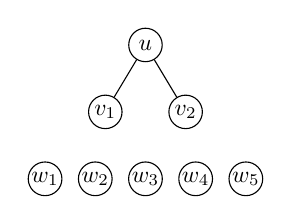
\begin{tikzpicture}[scale=0.85, every node/.style={scale=0.85,shape=circle,inner sep=.5pt,
                  minimum size=5mm}]
              \node[draw] (u) at (0,1) {$u$};
              \node[draw] (v1) at (-.6,0) {$v_1$};
              \node[draw] (v2) at (.6,0) {$v_2$};
              \node[draw] (w1) at (-1.5,-1) {$w_1$};
              \node[draw] (w2) at (-.75,-1) {$w_2$};
              \node[draw] (w3) at (0,-1) {$w_3$};
              \node[draw] (w4) at (.75,-1) {$w_4$};
              \node[draw] (w5) at (1.5,-1) {$w_5$};
              \draw (u) -- (v1);
              \draw (u) -- (v2);
          \end{tikzpicture}
        }
        \label{figure:gac-example-3}
    }
    \subfigure[][$H_2$] {
        \centering
        \scalebox{1}{
          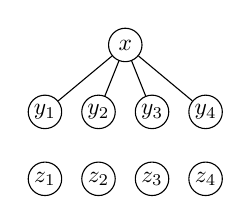
\begin{tikzpicture}[scale=0.85, every node/.style={scale=0.85,shape=circle,inner sep=.5pt,
                  minimum size=5mm}]
              \node[draw] (x) at (0,1) {$x$};
              \node[draw] (y1) at (-1.2,0) {$y_1$};
              \node[draw] (y2) at (-.4,0) {$y_2$};
              \node[draw] (y3) at (.4,0) {$y_3$};
              \node[draw] (y4) at (1.2,0) {$y_4$};
              \node[draw] (z1) at (-1.2,-1) {$z_1$};
              \node[draw] (z2) at (-.4,-1) {$z_2$};
              \node[draw] (z3) at (.4,-1) {$z_3$};
              \node[draw] (z4) at (1.2,-1) {$z_4$};
              \draw (x) -- (y1);
              \draw (x) -- (y2);
              \draw (x) -- (y3);
              \draw (x) -- (y4);
          \end{tikzpicture}
        }
        \label{figure:gac-example-4}
    }
    \subfigure[][$G_k$] {
        \centering
        \scalebox{1}{
          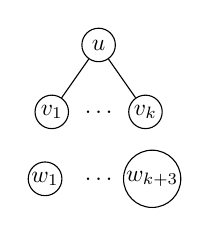
\begin{tikzpicture}[scale=0.85, every node/.style={scale=0.85,shape=circle,inner sep=.5pt,
                  minimum size=5mm}]
              \node[draw] (u) at (0,1) {$u$};
              \node[draw] (v1) at (-.7,0) {$v_1$};
              \node[] (vdots) at (0,0) {$\dots$};
              \node[draw] (v2) at (.7,0) {$v_k$};
              \node[draw] (w1) at (-.8,-1) {$w_1$};
              \node[] (wdots) at (0,-1) {$\dots$};
              \node[draw] (w5) at (.8,-1) {$w_{k+3}$};
              \draw (u) -- (v1);
              \draw (u) -- (v2);
          \end{tikzpicture}
        }
        \label{figure:gac-example-1}
    }
    \subfigure[][$H_k$] {
        \centering
        \scalebox{1}{
          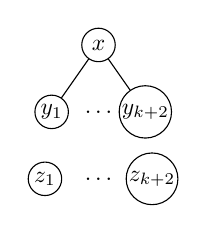
\begin{tikzpicture}[scale=0.85, every node/.style={scale=0.85,shape=circle,inner sep=.5pt,
                  minimum size=5mm}]
              \node[draw] (x) at (0,1) {$x$};
              \node[draw] (y1) at (-.7,0) {$y_1$};
              \node[] (ydots) at (0,0) {$\dots$};
              \node[draw] (y2) at (.7,0) {$y_{k+2}$};
              \node[draw] (z1) at (-.8,-1) {$z_1$};
              \node[] (zdots) at (0,-1) {$\dots$};
              \node[draw] (z5) at (.8,-1) {$z_{k+2}$};
              \draw (x) -- (y1);
              \draw (x) -- (y2);
          \end{tikzpicture}
        }
        \label{figure:gac-example-2}
    }
    \caption{Example graphs $G_2$ and $H_2$, and their generalised
    versions $G_k$ and $H_k$.}\label{figure:gac-example}
\end{figure}

When solving this instance, \McSplit-SI begins by mapping $u$ to $x$.  This leaves
two label classes:
$\langle \{v_1,v_2\}, \{y_1,y_2,y_3,y_4\} \rangle$
and
$\langle \{w_1,w_2,w_3,w_4,w_5\}, \{z_1,z_2,z_3,z_4\} \rangle$.  In the latter
label class, the set $V_G$ is larger than the set $V_H$, and therefore the
algorithm can backtrack and terminate.

Now we consider how the Glasgow algorithm behaves on this instance. After mapping
$u$ to $x$, the domains correspond to our label classes, as shown in the first two
columns of \Cref{tab:counting-all-diff}.  The remaining two columns of the table
illustrate the behaviour of the counting all-different propagator on these domains.
(Since all domains are of the same size, the stable sort function used by the algorithm
does not reorder the domains.)  The third column shows set $A$, which is the union
of domains in the current and previous rows.  The fourth column shows the number
of variables up to and including the current row.  Since $|A| \geq n$ on each row,
the propagator does not delete any values from the domains and does not conclude
that we can backtrack.

\begin{table}[htb]
\centering
\footnotesize
    \begin{tabular}{p{0.09\linewidth} p{0.16\linewidth} p{0.3\linewidth} p{0.08\linewidth}}
 \toprule
     Variable & Domain & $A$ & $n$\\ [0.5ex]
 \midrule
     $v_1$ & $\{y_1,y_2,y_3,y_4\}$ & $\{y_1,y_2,y_3,y_4\}$ & 1\\
     $v_2$ & $\{y_1,y_2,y_3,y_4\}$ & $\{y_1,y_2,y_3,y_4\}$ & 2\\
     $w_1$ & $\{z_1,z_2,z_3,z_4\}$ & $\{y_1,y_2,y_3,y_4,z_1,z_2,z_3,z_4\}$ & 3\\
     $w_2$ & $\{z_1,z_2,z_3,z_4\}$ & $\{y_1,y_2,y_3,y_4,z_1,z_2,z_3,z_4\}$ & 4\\
     $w_3$ & $\{z_1,z_2,z_3,z_4\}$ & $\{y_1,y_2,y_3,y_4,z_1,z_2,z_3,z_4\}$ & 5\\
     $w_4$ & $\{z_1,z_2,z_3,z_4\}$ & $\{y_1,y_2,y_3,y_4,z_1,z_2,z_3,z_4\}$ & 6\\
     $w_5$ & $\{z_1,z_2,z_3,z_4\}$ & $\{y_1,y_2,y_3,y_4,z_1,z_2,z_3,z_4\}$ & 7\\
%    $s_G$ & Pointer to Integer & Pointer to the first vertex of the $G$-set\\
%    \rule{0pt}{2.3ex}$e_G$ & Pointer to Integer & Pointer to one element past the last vertex of the $G$-set\\
 \bottomrule
\end{tabular}
\caption{A demonstration of the counting all-different propagator on $G_2$ and $H_2$
    after assigning $u$ to $x$.}
\label{tab:counting-all-diff}
\end{table}

The final two graphs in \Cref{figure:gac-example} generalise $G_2$ and $H_2$; as $k$ is incremented,
a vertex is added to each of the $v$, $w$, $y$ and $z$ sets.
\Cref{tab:gk-run-times} shows run times for the enumeration problem
using \McSplit-SI, Glasgow, Glasgow with no supplemental graphs, and RI for a range of values of
$k$.\footnote{VF3 was excluded from the experiment because the version available when the
experiment was run not handle disconnected graphs correctly.}
\McSplit-SI solves the instance $k=1\,000\,000$ in less than a second;
Glasgow and RI time out on the $k=10$ and $k=6$ instances respectively.

\begin{table}[htb]
\centering
\footnotesize
    \begin{tabular}{r r r r r}
 \toprule
        $k$ & \McSplit-SI & Glasgow & Glasgow-NS& RI \\ % [0.5ex]
 \midrule
        3 &  0 &  0 &  0 &  2\\
        4 &  0 &  0 &  0 &  86\\
        5 &  0 &  2 &  2 &  4305\\
        6 &  0 &  21 &  19 &  *\\
        7 &  0 &  195 &  191 &  *\\
        8 &  0 &  2083 &  1966 &  *\\
        9 &  0 &  24254 &  23443 &  *\\
        10 &  0 &  * &  * &  *\\
        10000 &  6 & * & * & *\\
        100000 &  66 & * & * & *\\
        1000000 &  676 & * & * & *\\
 \bottomrule
\end{tabular}
\caption{Run times in ms for the induced subgraph isomorphism enumeration problem on $G_k$ and $H_k$.
    An asterisk indicates timeout at 100 seconds. Glasgow-NS is the Glasgow Subgraph Solver
    with supplemental graphs disabled.}
\label{tab:gk-run-times}
\end{table}

\subsection{A family of instances where \McSplit-SI is outperformed by Glasgow}

In the previous subsection, we saw a family of instances on which \McSplit-SI outperforms
the Glasgow Subgraph Solver.  We can easily construct a family of instances where the reverse is true.
Consider the graphs in \Cref{figure:glasgow-fast-example}.
Graph $G'_3$ consists of three copies of the cycle $C_4$ and three copies of the star
$K_{1,3}$, with no additional edges.  Graph $H'_3$ consists of three copies of $C_5$
and three copies of $K_{1,3}$.  We generalise these definition to $G'_k$ and $H'_k$,
which have $k$ copies the cycle and star rather than 3.
For $k\geq 1$, no instance $(G'_k, H'_k)$ is satisfiable, since $H'_k$ does not contain
an induced 4-cycle.

The \McSplit-SI algorithm prefers to map high-degree vertices first, and therefore its first
decisions on these instances involves the stars rather than the cycles.  Only at deeper
levels of the search
tree, when all of the stars have been mapped, does the algorithm begin to work on the cycles,
at which point it can backtrack.  Unfortunately, there are $6^k k!$ ways to map the stars
of $G'_k$ to the stars of $H'_k$, since any star in the pattern graph can be mapped to any
star in the target graph and there are six possible ways to map the leaf nodes of any star.
Therefore \McSplit-SI's search tree is very large even
for small values of $k$.

With supplemental graphs disabled, the Glasgow algorithm suffers from the same problem.
However, supplemental graphs allow the Glasgow Subgraph Solver to solve these instances
without search.  In particular, consider the supplemental graph in which $v$ and $w$
are adjacent
if and only there are at least two 2-paths between $v$ and $w$ in the original graph.
This supplemental graph
contains edges between vertices of the 4-cycles in the pattern graph, but has no edges for the
target graph.

\Cref{tab:gk-prime-run-times} shows that supplemental graphs make a huge
difference to Glasgow's run times in practice on this family of instances.  The
table shows times for \McSplit-SI, Glasgow, Glasgow without supplemental
graphs, and RI.  \McSplit-SI and RI have similar run times, and cannot solve
instances with $k$ greater than 5 within the 100 second time limit.  Glasgow can
solve the instance with $k=1000$ (a 7000-vertex pattern graph and an
8000-vertex target graph) in less than 4 seconds.

\begin{figure}[htb]
    \centering
    \subfigure[][$G'_3$] {
        \centering
        \scalebox{1}{
          \foreach \n in {1,...,3}{
              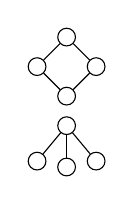
\begin{tikzpicture}[scale=0.75, every node/.style={scale=0.75,shape=circle,inner sep=.5pt,
                      minimum size=3mm}]
                  \node[draw] (a) at (0,0) {};
                  \node[draw] (b) at (.5,.5) {};
                  \node[draw] (c) at (1,0) {};
                  \node[draw] (d) at (.5,-.5) {};
                  \node[draw] (e) at (.5,-1) {};
                  \node[draw] (f) at (0,-1.6) {};
                  \node[draw] (g) at (.5,-1.7) {};
                  \node[draw] (h) at (1,-1.6) {};
                  \draw (a) -- (b) -- (c) -- (d) -- (a);
                  \draw (e) -- (f);
                  \draw (e) -- (g);
                  \draw (e) -- (h);
              \end{tikzpicture}
          }
        }
    }
    \subfigure[][$H'_3$] {
        \centering
        \scalebox{1}{
          \foreach \n in {1,...,3}{
              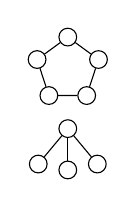
\begin{tikzpicture}[scale=0.75, every node/.style={scale=0.75,shape=circle,inner sep=.5pt,
                      minimum size=3mm}]
                  \node[draw] (z) at (0.5,0.55) {};
                  \node[draw] (a) at (-0.02,0.17) {};
                  \node[draw] (b) at (0.18,-0.44) {};
                  \node[draw] (c) at (0.82,-0.44) {};
                  \node[draw] (d) at (1.02,0.17) {};
                  \node[draw] (e) at (.5,-1) {};
                  \node[draw] (f) at (0,-1.6) {};
                  \node[draw] (g) at (.5,-1.7) {};
                  \node[draw] (h) at (1,-1.6) {};
                  \draw (a) -- (b) -- (c) -- (d) -- (z) -- (a);
                  \draw (e) -- (f);
                  \draw (e) -- (g);
                  \draw (e) -- (h);
              \end{tikzpicture}
          }
        }
    }
    \caption{Example graphs $G'_3$ and $H'_3$.}\label{figure:glasgow-fast-example}
\end{figure}

\begin{table}[htb]
\centering
\footnotesize
    \begin{tabular}{r r r r r}
 \toprule
     $k$ & \McSplit-SI & Glasgow & Glasgow-NS& RI \\ %[0.5ex]
 \midrule
     1 &  0 &  0 &  0 &  0\\
     2 &  0 &  0 &  1 &  0\\
     3 &  10 &  0 &  47 &  10\\
     4 &  329 &  0 &  1793 &  324\\
     5 &  12522 &  0 &  80880 &  11987\\
     6 &  * &  0 &  * &  *\\
     7 &  * &  0 &  * &  *\\
     8 &  * &  0 &  * &  *\\
     9 &  * &  0 &  * &  *\\
     10 &  * &  0 &  * &  *\\
     100 &  * &  27 &  * &  *\\
     1000 &  * &  3825 &  * &  *\\
 \bottomrule
\end{tabular}
\caption{Run times in ms for the induced subgraph isomorphism enumeration problem on $G'_k$ and $H'_k$.
    An asterisk indicates timeout at 100 seconds. Glasgow-NS is the Glasgow Subgraph Solver
    with supplemental graphs disabled.}
\label{tab:gk-prime-run-times}
\end{table}

As we have seen in this section, neither \McSplit-SI nor Glasgow dominates the other solver.  In the next
section, we perform an experimental evalulation to compare solvers on benchmark instances.

\section{Experimental evaluation}\label{sec:mcsplit-si-experiments}
\label{sec:si-experiments}

We now compare the speed of \McSplit-SI with existing state-of-the-art algorithms
on three sets of benchmark instances.  \Cref{subsec:si-decision-experiment}
uses an existing large, heterogeneous set of pairs of unlabelled
graphs.
In \Cref{subsec:si-knights-experiment},
we consider a new set of decision-problem
instances recently proposed by Donald Knuth based on a generalisation of the knight's
tour problem.
Finally, in \Cref{subsec:si-enumeration-experiment}, we use pairs of random directed
graphs based on another existing benchmark set;
we solve the problem of counting all induced subgraph isomorphisms from the pattern to the target.

\subsection{Solvers used}

Our experiments compare \McSplit-SI with four state-of-the-art subgraph isomorphism solvers:
VF3, RI, RI-DS, and Glasgow.   In addition, we use PathLAD in \Cref{subsec:si-knights-experiment};
this solver has been shown in prior work to be outperformed by Glasgow and VF3 respectively
on the other two sets of instances \citep{DBLP:journals/pami/CarlettiFSV18,DBLP:conf/gbrpr/Solnon19}.
These solvers are described in \Cref{sec:si-algorithms}.
In terms of effort per search node, \McSplit-SI may be viewed intuitively as sitting
between Glasgow and PathLAD on one hand and VF3, RI, and RI-DS on the other.

We use the 14 March 2022 version of the Glasgow solver, published
online.\footnote{\url{https://github.com/ciaranm/glasgow-subgraph-solver}}
In addition, we report results of the Glasgow solver with supplemental graphs
switched off.

The \McSplit-SI variants used are shown in \Cref{tab:mcsplit-si-variants}.

\begin{table}[htb]
\centering
\footnotesize
 \begin{tabular}{p{0.18\linewidth} p{0.75\linewidth} }
 \toprule
    Name & Description \\ [0.5ex]
 \midrule
    \McSplit-SI & The base \McSplit-SI algorithm \\
    \rule{0pt}{2.3ex}\McSplit-SI-LL & \McSplit-SI with lists of vertices stored as sorted doubly-linked lists
                (\Cref{sec:mcsplit-si-ll})\\
    \rule{0pt}{2.3ex}\McSplit-SI-AM & An adaptation of \McSplit\ decision-problem solver (using adjacence matrix
        representation of graphs) to the induced subgraph isomorphism problem.  This does not use \McSplit-SI's
        partitioning algorithm optimised for sparse graphs. (\Cref{sec:mcsplit-si-adjmat})\\
    \rule{0pt}{2.3ex}\McSplit-SI-static & \McSplit-SI with the dynamic variable-ordering heuristic replaced by
        the static heuristic of RI \citep{DBLP:journals/tcbb/BonniciG17} (\Cref{subsec:mcsplit-si-static})\\
%    \rule{0pt}{2.3ex}\McSplit-SI-pre & TODO, refer forward. \\
\bottomrule
\end{tabular}
\caption{Summary of \McSplit-SI variants used in this chapter's experiments}
\label{tab:mcsplit-si-variants}
\end{table}

\subsection{Decision instances}\label{subsec:si-decision-experiment}

Our first set of benchmark instances is
a collection of $14,621$ pairs of undirected, unlabelled graphs.
This collection was used by \citet{DBLP:conf/cpaior/ArchibaldDHMP019},
extending the work of \citet{DBLP:conf/lion/KotthoffMS16};
it assembles instances from several smaller benchmarks.

\paragraph*{Families of instances} The benchmark set contains graphs
in the following families.

\begin{itemize}
    \item
        \textbf{Scalefree:} Randomly generated scale-free graphs \citep{DBLP:books/daglib/0012457}: 80
        satisfiable instances and 20 unsatisfiable instances.  In each instance,
        $|V(G)| = 0.9 \times |V(H)|$. Source: \citet{DBLP:journals/constraints/ZampelliDS10}
    \item
        \textbf{LV:} Pairs of graphs derived from the Stanford GraphBase \citep{DBLP:books/daglib/0071477}.
        Source: \cite{DBLP:journals/mscs/LarrosaV02}.
    \item \textbf{BVG:} Regular and irregular bounded valence target graphs, randomly generated.
        In the regular instances, the vertices of the target graph have equal degree of 3, 6, or 9
        depending on the instance.  The irregular instances have variable degree but a fixed total
        number of edges.
        This and the following two families are from the database
        of instances described in \citet{DBLP:journals/prl/SantoFSV03}.  For each instance in these
        three families, the pattern graphs were generated by taking a random connected
        induced subgraph of the target graph. All instances in these families are therefore satisfiable.
    \item \textbf{M4D:} Regular and irregular 4-dimensional meshes.  The irregular instances have
        extra edges added to the mesh graph.
    \item \textbf{Rand:} Erd\H{o}s-Rényi $G(n,p)$ random graphs.
    \item \textbf{Phase:} Pairs of Erd\H{o}s-Rényi $G(n,p)$ random graphs
        with parameters chosen near the satisfiable/unsatifiable phase transition in order
        to make the instances very challenging to solve.
        \citep{DBLP:journals/jair/McCreeshPST18}
    \item \textbf{PR}, \textbf{Meshes} and \textbf{Images:} Instances derived from a pattern recognition problem, where
    	the graphs are generated from the adjacencies of regions of an image (PR, Images)
	or 3D object model (Meshes). \citep{DBLP:journals/pr/SolnonDHJ15,DBLP:journals/cviu/DamiandSHJS11}
\end{itemize}

\Cref{tab:instance-family-summary} shows a summary of the instances in each family.
Most of the graphs are sparse; the LV and Phase families are unusual in that they contain
some very dense target graphs.

\begin{table}[htb]
\centering
\footnotesize
    \begin{tabular}{lrrrrrrrrr}
 \toprule
        Family & Count & \multicolumn{4}{c}{Pattern graph} & \multicolumn{4}{c}{Target graph} \\
     \cmidrule(r){3-6}
     \cmidrule(r){7-10}
             & & $n_{\min{}}$ & $n_{\max{}}$ & $d_{\min{}}$ & $d_{\max{}}$
            & $n_{\min{}}$ & $n_{\max{}}$ & $d_{\min{}}$ & $d_{\max{}}$
            \\ [0.5ex]
 \midrule
        \rule{0pt}{2.3ex}Scalefree & 100 & 180 & 900 & 0.0060 & 0.1646 & 200 & 1000 & 0.0060 & 0.1594 \\
\rule{0pt}{2.3ex}LV & 3831 & 10 & 128 & 0.0198 & 1.0000 & 10 & 6671 & 0.0006 & 1.0000 \\
\rule{0pt}{2.3ex}BVG & 540 & 40 & 480 & 0.0055 & 0.2013 & 200 & 800 & 0.0037 & 0.0452 \\
\rule{0pt}{2.3ex}M4D & 360 & 51 & 777 & 0.0045 & 0.0839 & 256 & 1296 & 0.0043 & 0.0253 \\
\rule{0pt}{2.3ex}Rand & 270 & 40 & 360 & 0.0201 & 0.2090 & 200 & 600 & 0.0201 & 0.1915 \\
\rule{0pt}{2.3ex}PR & 24 & 4 & 170 & 0.0168 & 0.6667 & 4838 & 4838 & 0.0006 & 0.0006 \\
\rule{0pt}{2.3ex}Phase & 200 & 30 & 30 & 0.2943 & 0.8897 & 150 & 150 & 0.3698 & 0.7821 \\
\rule{0pt}{2.3ex}Meshes & 3018 & 40 & 199 & 0.0219 & 0.1462 & 201 & 5873 & 0.0004 & 0.0224 \\
\rule{0pt}{2.3ex}Images & 6278 & 15 & 151 & 0.0186 & 0.1905 & 1072 & 5972 & 0.0005 & 0.0027 \\

%    1 & 100 & \numrange{200}{1000} & w  \\
%    \rule{0pt}{2.3ex}X & x & y & z \\
 \bottomrule
\end{tabular}
    \caption{Summary of instance families. The values $n_{\min{}}$ and $n_{\max{}}$
            are the smallest and largest vertex counts; the values $d_{\min{}}$ and $d_{\max{}}$
            are the smallest and largest densities.}
\label{tab:instance-family-summary}
\end{table}

%%     plotfile u (c(xcol)==0&&c(ycol)==0?NaN:column(famcol)!=1?NaN:clamp(xcol)):(clamp(ycol)) ls 1 pt 1 ps 0.7 ti 'SF', \
%%     plotfile u (c(xcol)==0&&c(ycol)==0?NaN:(column(famcol)!=2&&column(famcol)!=11)?NaN:clamp(xcol)):(clamp(ycol)) w p ls 2 pt 2 ps 0.7 ti 'LV', \
%%     plotfile u (c(xcol)==0&&c(ycol)==0?NaN:(column(famcol)!=3&&column(famcol)!=4)?NaN:clamp(xcol)):(clamp(ycol)) ls 3 pt 3 ps 0.7 ti 'BVG(r)', \
%%     plotfile u (c(xcol)==0&&c(ycol)==0?NaN:(column(famcol)!=5&&column(famcol)!=6)?NaN:clamp(xcol)):(clamp(ycol)) ls 4 pt 4 ps 0.7 ti 'M4D(r)', \
%%     plotfile u (c(xcol)==0&&c(ycol)==0?NaN:column(famcol)!=7?NaN:clamp(xcol)):(clamp(ycol)) ls 5 pt 10 ps 0.7 ti 'Rand', \
%%     plotfile u (c(xcol)==0&&c(ycol)==0?NaN:column(famcol)!=9?NaN:clamp(xcol)):(clamp(ycol)) ls 6 pt 6 ps 0.7 ti 'PR', \
%%     plotfile u (c(xcol)==0&&c(ycol)==0?NaN:column(famcol)!=12?NaN:clamp(xcol)):(clamp(ycol)) ls 7 pt 8 ps 0.7 ti 'Phase', \
%%     plotfile u (c(xcol)==0&&c(ycol)==0?NaN:column(famcol)!=13?NaN:clamp(xcol)):(clamp(ycol)) ls 13 pt 14 ps 0.7 ti 'Meshes', \
%%     plotfile u (c(xcol)==0&&c(ycol)==0?NaN:column(famcol)!=14?NaN:clamp(xcol)):(clamp(ycol)) ls 8 pt 12 ps 0.7 ti 'Images', \
\paragraph*{Results}

\Cref{figure:unlabelled-vf-instance-runtimes} shows cumulative plots of instances solved by \McSplit-SI
and the other algorithms.  To avoid a tangle of overlapping curves, each solver's curve is shown as a dark
blue line on its own plot, with the curve for \McSplit-SI shown in light blue for comparison on each
plot.  The solvers can be split into three broad categories.  Constraint programming solvers tend
to run slowly on the easiest instances but perform well for hard instances.  The two versions of Glasgow
are in this category; \McSplit-SI-AM has similar results.  Pattern recognition solvers---RI and VF3
in particular---perform well on easy instances but solve fewer of the hard instances than the constraint
programming solvers;
\citet{DBLP:conf/gbrpr/Solnon19} makes a similar observation for these two solver categories.
Finally, \McSplit-SI and \McSplit-SI-LL perform well on easy instances---indeed, outperforming
the pattern recognition solvers---while solving almost as many of the hard instances as Glasgow.

\begin{figure}[htb]
    \centering
    \subfigure[][Glasgow] {
        \includegraphics*[width=0.22\textwidth]{14b-mcsplit-induced-si/decision-instances-experiment/experiment/plots/cumulative-mcsplit-glasgow}
        \label{figure:TODO}
    }
    \subfigure[][Glasgow, no supp.] {
        \includegraphics*[width=0.22\textwidth]{14b-mcsplit-induced-si/decision-instances-experiment/experiment/plots/cumulative-mcsplit-glasgow-nosupp}
        \label{figure:TODO}
    }
    \subfigure[][RI] {
        \includegraphics*[width=0.22\textwidth]{14b-mcsplit-induced-si/decision-instances-experiment/experiment/plots/cumulative-mcsplit-ri}
        \label{figure:TODO}
    }
    \subfigure[][RI-DS] {
        \includegraphics*[width=0.22\textwidth]{14b-mcsplit-induced-si/decision-instances-experiment/experiment/plots/cumulative-mcsplit-ri-ds}
        \label{figure:TODO}
    }
    \subfigure[][VF3] {
        \includegraphics*[width=0.22\textwidth]{14b-mcsplit-induced-si/decision-instances-experiment/experiment/plots/cumulative-mcsplit-vf3}
        \label{figure:TODO}
    }
    \subfigure[][\McSplit-SI-LL] {
        \includegraphics*[width=0.22\textwidth]{14b-mcsplit-induced-si/decision-instances-experiment/experiment/plots/cumulative-mcsplit-si-ll}
        \label{figure:TODO}
    }
    \subfigure[][\McSplit-SI-AM] {
        \includegraphics*[width=0.22\textwidth]{14b-mcsplit-induced-si/decision-instances-experiment/experiment/plots/cumulative-mcsplit-si-am}
        \label{figure:TODO}
    }
    \caption{Cumulative plots of run times for decision instances.  In each subfigure, the algorithm named
        in the caption is in dark blue and \McSplit-SI is in light blue.}
    \label{figure:unlabelled-vf-instance-runtimes}
\end{figure}

\Cref{figure:si-decision-scatter} shows a scatter plot of run times for each solver, with the run time of
\McSplit-SI on the horizontal axis in each plot.  \McSplit-SI compares favourably
to each of the non-\McSplit\ solvers in the first five plots, although each of these has some instances that it can solve
in less than a second while \McSplit-SI exceeds the time limit; this is likely to be due to a combination
of different variable and value ordering heuristics and, in the case of Glasgow, stronger filtering.

\begin{figure}[htb]
    \centering
    \subfigure[][Glasgow] {
        \includegraphics*[width=0.22\textwidth]{14b-mcsplit-induced-si/decision-instances-experiment/experiment/plots/scatter-mcsplit-glasgow}
        \label{figure:TODO}
    }
    \subfigure[][Glasgow, no supp.] {
        \includegraphics*[width=0.22\textwidth]{14b-mcsplit-induced-si/decision-instances-experiment/experiment/plots/scatter-mcsplit-glasgow-nosupp}
        \label{figure:TODO}
    }
    \subfigure[][RI] {
        \includegraphics*[width=0.22\textwidth]{14b-mcsplit-induced-si/decision-instances-experiment/experiment/plots/scatter-mcsplit-ri}
        \label{figure:TODO}
    }
    \subfigure[][RI-DS] {
        \includegraphics*[width=0.22\textwidth]{14b-mcsplit-induced-si/decision-instances-experiment/experiment/plots/scatter-mcsplit-ri-ds}
        \label{figure:TODO}
    }
    \subfigure[][VF3] {
        \includegraphics*[width=0.22\textwidth]{14b-mcsplit-induced-si/decision-instances-experiment/experiment/plots/scatter-mcsplit-vf3}
        \label{figure:TODO}
    }
    \subfigure[][\McSplit-SI-LL] {
        \includegraphics*[width=0.22\textwidth]{14b-mcsplit-induced-si/decision-instances-experiment/experiment/plots/scatter-mcsplit-si-ll}
        \label{figure:TODO}
    }
    \subfigure[][\McSplit-SI-AM] {
        \includegraphics*[width=0.22\textwidth]{14b-mcsplit-induced-si/decision-instances-experiment/experiment/plots/scatter-mcsplit-si-am}
        \label{figure:TODO}
    }
    \caption{Scatter plots of run times in ms for decision instances.
            The horizontal and vertical axes show the run times of \McSplit-SI and the
            solver named in the subfigure caption, respectively.}
    \label{figure:si-decision-scatter}
\end{figure}

TODO: mention that D1 variant isn't very good.
TODO: mention that D2 variant has similar results to Glasgow on phase instances.

\FloatBarrier

To give a finer-grained look at the performance of the two best solvers overall---\McSplit-SI and
Glasgow---\Cref{figure:mcsplitsi-scatter-by-family} shows those solvers' run times for each
instance, with a separate sub-figure for each family of instances.  On the PR, Phase, Meshes,
and Images families, \McSplit-SI is the clear winner.   On each of
the remaining five families, \McSplit-SI is the faster solver on most instances, but Glasgow
is much faster than \McSplit-SI on a small proportion of instances.

\begin{figure}[htb]
    \centering
    \subfigure[][Scalefree] {
        \includegraphics*[width=0.22\textwidth]{14b-mcsplit-induced-si/decision-instances-experiment/experiment/plots/by-family/scatter-Scalefree.pdf}
        \label{figure:TODO}
    }
    \subfigure[][LV] {
        \includegraphics*[width=0.22\textwidth]{14b-mcsplit-induced-si/decision-instances-experiment/experiment/plots/by-family/scatter-LV.pdf}
        \label{figure:TODO}
    }
    \subfigure[][BVG] {
        \includegraphics*[width=0.22\textwidth]{14b-mcsplit-induced-si/decision-instances-experiment/experiment/plots/by-family/scatter-BVG.pdf}
        \label{figure:TODO}
    }

    \subfigure[][M4D] {
        \includegraphics*[width=0.22\textwidth]{14b-mcsplit-induced-si/decision-instances-experiment/experiment/plots/by-family/scatter-M4D.pdf}
        \label{figure:TODO}
    }
    \subfigure[][Rand] {
        \includegraphics*[width=0.22\textwidth]{14b-mcsplit-induced-si/decision-instances-experiment/experiment/plots/by-family/scatter-Rand.pdf}
        \label{figure:TODO}
    }
    \subfigure[][PR] {
        \includegraphics*[width=0.22\textwidth]{14b-mcsplit-induced-si/decision-instances-experiment/experiment/plots/by-family/scatter-PR.pdf}
        \label{figure:TODO}
    }

    \subfigure[][Phase] {
        \includegraphics*[width=0.22\textwidth]{14b-mcsplit-induced-si/decision-instances-experiment/experiment/plots/by-family/scatter-Phase.pdf}
        \label{figure:TODO}
    }
    \subfigure[][Meshes] {
        \includegraphics*[width=0.22\textwidth]{14b-mcsplit-induced-si/decision-instances-experiment/experiment/plots/by-family/scatter-Meshes.pdf}
        \label{figure:TODO}
    }
    \subfigure[][Images] {
        \includegraphics*[width=0.22\textwidth]{14b-mcsplit-induced-si/decision-instances-experiment/experiment/plots/by-family/scatter-Images.pdf}
        \label{figure:TODO}
    }
    \caption{Run times in ms of \McSplit-SI (horizontal axis) and Glasgow (vertical axis), by family.}
    \label{figure:mcsplitsi-scatter-by-family}
\end{figure}

On an instance-by-instance basis, does \McSplit-SI typically run faster than
the best of the other solvers? To answer this question, we calculate the run
time of the virtual best other solver (VBOS) for each instance
by taking the lowest run time
of the five non-\McSplit\ solvers: Glasgow, Glasgow without supplemental graphs, RI, RI-DS, and VF3.
This VBOS is essentially equivalent to running the constitutent solvers in parallel
and stopping when the first solver terminates; we can also view it
as an idealised portfolio solver with an oracle that selects
the best non-\McSplit\ solver for a given instance.

\Cref{figure:mcsplitsi-vbs-scatter-by-family} shows the run times of \McSplit-SI
and VBOS (vertical axis) for each instance.  On six families
of instances (BVG, Rand, LV, Phase, Images, Meshes), the number
of instances where \McSplit-SI is faster than VBOS is greater than the number of instances where
the reverse is true. 
On the other hand, \McSplit-SI certainly does not dominate the other solvers;
indeed, there are families such as Scalefree where \McSplit-SI appears to be worse overall than VBOS.

\begin{figure}[htb]
    \centering
    \subfigure[][Scalefree] {
        \includegraphics*[width=0.22\textwidth]{14b-mcsplit-induced-si/decision-instances-experiment/experiment/plots/by-family/scatter-Scalefree-vbos.pdf}
        \label{figure:TODO}
    }
    \subfigure[][LV] {
        \includegraphics*[width=0.22\textwidth]{14b-mcsplit-induced-si/decision-instances-experiment/experiment/plots/by-family/scatter-LV-vbos.pdf}
        \label{figure:TODO}
    }
    \subfigure[][BVG] {
        \includegraphics*[width=0.22\textwidth]{14b-mcsplit-induced-si/decision-instances-experiment/experiment/plots/by-family/scatter-BVG-vbos.pdf}
        \label{figure:TODO}
    }

    \subfigure[][M4D] {
        \includegraphics*[width=0.22\textwidth]{14b-mcsplit-induced-si/decision-instances-experiment/experiment/plots/by-family/scatter-M4D-vbos.pdf}
        \label{figure:TODO}
    }
    \subfigure[][Rand] {
        \includegraphics*[width=0.22\textwidth]{14b-mcsplit-induced-si/decision-instances-experiment/experiment/plots/by-family/scatter-Rand-vbos.pdf}
        \label{figure:TODO}
    }
    \subfigure[][PR] {
        \includegraphics*[width=0.22\textwidth]{14b-mcsplit-induced-si/decision-instances-experiment/experiment/plots/by-family/scatter-PR-vbos.pdf}
        \label{figure:TODO}
    }

    \subfigure[][Phase] {
        \includegraphics*[width=0.22\textwidth]{14b-mcsplit-induced-si/decision-instances-experiment/experiment/plots/by-family/scatter-Phase-vbos.pdf}
        \label{figure:TODO}
    }
    \subfigure[][Meshes] {
        \includegraphics*[width=0.22\textwidth]{14b-mcsplit-induced-si/decision-instances-experiment/experiment/plots/by-family/scatter-Meshes-vbos.pdf}
        \label{figure:TODO}
    }
    \subfigure[][Images] {
        \includegraphics*[width=0.22\textwidth]{14b-mcsplit-induced-si/decision-instances-experiment/experiment/plots/by-family/scatter-Images-vbos.pdf}
        \label{figure:TODO}
    }
    \caption{Run times in ms of \McSplit-SI (horizontal axis) and the virtual best other solver (vertical axis), by family.}
    \label{figure:mcsplitsi-vbs-scatter-by-family}
\end{figure}

\FloatBarrier

\paragraph*{The effect of target graph density}
When is it better to use \McSplit-SI than \McSplit-SI-AM?
\Cref{figure:density-runtime-ratio-am} has a point per instance, with target graph density on the x axis and the ratio of the two solvers' run times 
on the y axis; a ratio below 1 indicates that \McSplit-SI is the faster solver.  Trivial instances and instances where at least one
solver timed out are excluded.  There is a clear positive relationship between density and ratio of run times.  For most instances of
density below $0.002$, \McSplit-SI is more than $10$ times faster than \McSplit-SI-AM.  However,
\McSplit-SI-AM soon begins to catch up as target graph density increases, and becomes the faster solver at a target graph density of around
$0.1$.\footnote{This analysis was carried out using target graph density because we would expect the target graph to have
a larger effect on run times than the (smaller) pattern graph.  We also re-created the plot with the x axis showing the proportion
of all possible edges across pattern \emph{and} target graphs: $(m_G + m_H) / (n_G(n_G-1) + n_H(n_H-1))$,
where $m_G$ and $n_G$ denote the edge and vertex counts of $G$.  The resulting
plot was almost identical to \Cref{figure:density-runtime-ratio-am}.}

\Cref{figure:density-runtime-ratio-glasgow} is a similar plot comparing the run time of \McSplit-SI to that of Glasgow.
(Note the larger range of values of the y axis.)  For very sparse target graphs with density below around $0.002$,
\McSplit-SI consistently runs faster than Glasgow---often by more than an order of magnitude.  For most of the
instances with denser target graphs,
\McSplit-SI is again the faster algorithm, and this holds true even for very dense graphs which are not well suited
to \McSplit-SI's data structures.  However, there is a long tail of instances
for which a combination of Glasgow's restarts and stronger filtering methods results in
an orders-of-magnitude speedup over \McSplit-SI.

\begin{figure}[htb]
    \centering
    \subfigure[][\McSplit-SI-AM] {
        \includegraphics*[width=0.5\textwidth]{14b-mcsplit-induced-si/decision-instances-experiment/experiment/plots/density-runtime-ratio}
        \label{figure:density-runtime-ratio-am}
    }\subfigure[][Glasgow] {
        \includegraphics*[width=0.5\textwidth]{14b-mcsplit-induced-si/decision-instances-experiment/experiment/plots/density-runtime-ratio-glasgow}
        \label{figure:density-runtime-ratio-glasgow}
    }
    \caption{On the horizontal axis, the target graph density; on the vertical axis, the ratio of \McSplit-SI run time to
            the run time of the algorithm named in the subfigure caption.
            Instances where either solver took less than 1 ms or exceeded the time limit are excluded.}
    \label{figure:density-runtime-ratio}
\end{figure}

\FloatBarrier

\paragraph*{Presolve} \cite{DBLP:conf/gbrpr/Solnon19} considers a solver that
runs VF3 for 100 ms, then switches to Glasgow if a solution is not found. This
outperforms Glasgow on easy instances while retaining almost all of the benefit
of Glasgow on hard instances.  Are there pairs of solvers in our experiment
that work particularly well using such a 100 ms presolve?
\Cref{tab:si-decision-presolve-counts} shows the number of instances solved
within 1000 seconds by each pair of solvers, excluding \McSplit-SI-AM and RI-DS
to save space.  Seven pairs of solvers---each of which used a version of \McSplit-SI
as the presolver, the main solver, or both---solved more instances than Glasgow,
which was the single
best individal solver by this measure with $14,524$ instances solved.
The best two solver pairs
each solved $14,546$ instances.  These use \McSplit-SI-static as the main
solver and either \McSplit-SI or Glasgow without supplemental graphs as the
presolver.

\begin{table}[htb]
\centering
\footnotesize
    
\begin{tabular}{lrrrrrr}
    \toprule

 & McS-SI & McS-SI-s & Gla & Gla, no supp. & RI & VF3 \\

    \midrule

McS-SI &  & $\underline{14\,546}$ & $\underline{14\,526}$ & $14\,498$ & $14\,277$ & $14\,251$ \\
McS-SI-s & $\underline{14\,535}$ &  & $\underline{14\,526}$ & $14\,512$ & $14\,068$ & $14\,141$ \\
Gla & $\underline{14\,537}$ & $14\,513$ &  & $14\,510$ & $14\,055$ & $14\,113$ \\
Gla, no supp. & $14\,524$ & $\underline{14\,546}$ & $14\,524$ &  & $14\,252$ & $14\,212$ \\
RI & $\underline{14\,528}$ & $14\,511$ & $14\,524$ & $14\,504$ &  & $14\,071$ \\
VF3 & $14\,510$ & $14\,510$ & $14\,524$ & $14\,496$ & $13\,976$ &  \\

    \bottomrule
\end{tabular}


\caption{Number of instances solved within 1000 seconds using a 100 ms presolve.  Each number
        refers to a solver that runs the solver named in the row for 100 ms, then switches to the
        solver named in the column.  Underlined values are greater than the number of instances
        solved by Glasgow without presolve ($14,524$). McS-SI-s=\McSplit-SI-static.}
\label{tab:si-decision-presolve-counts}
\end{table}

\paragraph*{Number of instances solved}
\Cref{tab:si-decision-solved-counts} shows, for each family and each solver,
the number of instances that were solved within the 1000-second time limit.
The final column, ``McS pre.'', refers to a solver that runs \McSplit-SI for 100 ms
as a presolver, then runs \McSplit-SI-static for the remaining time.  For every
family, this solver is able to solve at least as many instances as the best other
solver.

``Phase'' is family on which all \McSplit-SI variants perform particularly well in
\Cref{tab:si-decision-solved-counts}.  This family is unusual in that the graphs
in many of the instances have density greater than $\nicefrac{1}{2}$.  
Much of the success of \McSplit-SI on these instances is due to the
strategy of sorting graphs in increasing order of degree if the target
graph is dense (\Cref{sec:mcsplit-si-heuristics}).  I re-ran the experiment 
with \McSplit-SI using the decreasing-degree sort order for all graphs;
only 179 rather than 199 Phase instances were solved within the time limit.

\begin{table}[htb]
\centering
\footnotesize
    
\begin{tabular}{crrrrrrrr}
    \toprule
    Family & Count & McS-SI & McS-SI-LL & Gla & Gla, no supp. & RI & VF3 & McS pre.\\
    \midrule

1 & $100$ & $\underline{100}$ & $\underline{100}$ & $\underline{100}$ & $\underline{100}$ & $90$ & $98$ & $\underline{100}$\\
2 & $793$ & $\underline{793}$ & $\underline{793}$ & $789$ & $786$ & $708$ & $726$ & $791$\\
3 & $270$ & $\underline{270}$ & $\underline{270}$ & $\underline{270}$ & $\underline{270}$ & $\underline{270}$ & $\underline{270}$ & $\underline{270}$\\
4 & $270$ & $\underline{270}$ & $\underline{270}$ & $\underline{270}$ & $\underline{270}$ & $267$ & $269$ & $\underline{270}$\\
5 & $90$ & $89$ & $89$ & $\underline{90}$ & $\underline{90}$ & $\underline{90}$ & $87$ & $\underline{90}$\\
6 & $270$ & $\underline{270}$ & $\underline{270}$ & $\underline{270}$ & $\underline{270}$ & $\underline{270}$ & $\underline{270}$ & $\underline{270}$\\
7 & $270$ & $259$ & $259$ & $\underline{270}$ & $260$ & $263$ & $263$ & $\underline{270}$\\
9 & $24$ & $\underline{24}$ & $\underline{24}$ & $\underline{24}$ & $\underline{24}$ & $\underline{24}$ & $\underline{24}$ & $\underline{24}$\\
11 & $3\,038$ & $2\,939$ & $2\,938$ & $\underline{2\,967}$ & $2\,950$ & $2\,904$ & $2\,863$ & $2\,966$\\
12 & $200$ & $\underline{199}$ & $\underline{199}$ & $178$ & $179$ & $5$ & $4$ & $\underline{199}$\\
13 & $3\,018$ & $\underline{3\,018}$ & $\underline{3\,018}$ & $\underline{3\,018}$ & $\underline{3\,018}$ & $2\,781$ & $2\,914$ & $\underline{3\,018}$\\
14 & $6\,278$ & $\underline{6\,278}$ & $\underline{6\,278}$ & $\underline{6\,278}$ & $\underline{6\,278}$ & $\underline{6\,278}$ & $\underline{6\,278}$ & $\underline{6\,278}$\\
TOTAL & $14\,621$ & $14\,509$ & $14\,508$ & $14\,524$ & $14\,495$ & $13\,950$ & $14\,066$ & $\underline{14\,546}$\\

    \bottomrule
\end{tabular}


\caption{The number of instances in each family that were solved by each solver
    within the 1000 second time limit.
    The ``Count'' column shows the total number of instances per family.
    An underlined value indicates that no other solver solved a greater number of instances
    in this family.}
\label{tab:si-decision-solved-counts}
\end{table}

\paragraph*{Number of instances for which each solver was the fastest}
\Cref{tab:si-decision-winner-counts} shows, for each family and each solver,
the number of instances for which the solver was the fastest of all solvers
shown.  For seven of the nine families, \McSplit-SI had the highest count
of ``wins''.  Glasgow performs poorly by this measure; for five families,
there were no instances for which it was the fastest solver.

\begin{table}[htb]
\centering
\footnotesize
    
\begin{tabular}{crrrrrrrr}
    \toprule
    Family & Count & McS-SI & McS-SI-LL & Gla & Gla, no supp. & RI & VF3 & McS + pre.\\
    \midrule

1 & $100$ & $61$ & $48$ & $0$ & $0$ & $60$ & $39$ & $\underline{64}$\\
2 & $793$ & $651$ & $\underline{670}$ & $284$ & $379$ & $214$ & $220$ & $632$\\
3 & $270$ & $\underline{270}$ & $252$ & $0$ & $4$ & $\underline{270}$ & $230$ & $231$\\
4 & $270$ & $\underline{248}$ & $228$ & $0$ & $12$ & $221$ & $190$ & $217$\\
5 & $90$ & $\underline{67}$ & $62$ & $3$ & $0$ & $49$ & $5$ & $42$\\
6 & $270$ & $164$ & $159$ & $2$ & $0$ & $\underline{218}$ & $125$ & $161$\\
7 & $270$ & $128$ & $47$ & $12$ & $1$ & $31$ & $17$ & $\underline{171}$\\
9 & $24$ & $19$ & $19$ & $0$ & $0$ & $20$ & $18$ & $\underline{22}$\\
11 & $3\,038$ & $\underline{2\,464}$ & $2\,185$ & $730$ & $1\,066$ & $1\,838$ & $1\,435$ & $2\,369$\\
12 & $200$ & $\underline{198}$ & $1$ & $0$ & $0$ & $0$ & $0$ & $0$\\
13 & $3\,018$ & $\underline{3\,000}$ & $2\,884$ & $617$ & $1\,147$ & $2\,468$ & $1\,754$ & $2\,692$\\
14 & $6\,278$ & $4\,794$ & $4\,104$ & $0$ & $0$ & $4\,196$ & $3\,524$ & $\underline{5\,094}$\\
TOTAL & $14\,621$ & $\underline{12\,064}$ & $10\,659$ & $1\,648$ & $2\,609$ & $9\,585$ & $7\,557$ & $11\,695$\\

    \bottomrule
\end{tabular}


\caption{For each family of instances, the number of instances for which each solver's
    run time equalled the best run time among all solvers shown.  The second
    column shows the total number of instances per family.  Underlined values
    are the best (or join-best) for that family.}
\label{tab:si-decision-winner-counts}
\end{table}

%% \begin{figure}[h!]
%%     \centering
%%     \includegraphics*[width=0.7\textwidth]{14b-mcsplit-induced-si/decision-instances-experiment/experiment/plots/cumulative-presolve}
%%     \caption{cumulative-presolve}
%%     \label{figure:cumulative-presolve}
%% \end{figure}
%% 
%% \begin{figure}[h!]
%%     \centering
%%     \includegraphics*[width=0.7\textwidth]{14b-mcsplit-induced-si/decision-instances-experiment/experiment/plots/cumulative}
%%     \caption{cumulative}
%%     \label{figure:cumulative}
%% \end{figure}
%% 
%% \begin{figure}[h!]
%%     \centering
%%     \includegraphics*[width=0.7\textwidth]{14b-mcsplit-induced-si/decision-instances-experiment/experiment/plots/sat-cumulative}
%%     \caption{sat-cumulative}
%%     \label{figure:sat-cumulative}
%% \end{figure}
%% 
%% \begin{figure}[h!]
%%     \centering
%%     \includegraphics*[width=0.7\textwidth]{14b-mcsplit-induced-si/decision-instances-experiment/experiment/plots/unsat-cumulative}
%%     \caption{unsat-cumulative}
%%     \label{figure:unsat-cumulative}
%% \end{figure}
%% 
%% \begin{figure}[h!]
%%     \centering
%%     \includegraphics*[width=0.7\textwidth]{14b-mcsplit-induced-si/decision-instances-experiment/experiment/plots/cumulative-without-disconnected-instances}
%%     \caption{cumulative-without-disconnected-instances}
%%     \label{figure:cumulative-without-disconnected-instances}
%% \end{figure}
%% 
%% \begin{figure}[h!]
%%     \centering
%%     \includegraphics*[width=0.45\textwidth]{14b-mcsplit-induced-si/decision-instances-experiment/experiment/plots/mcsplit-si-vs-adjmat}
%%     \caption{mcsplit-si-vs-adjmat}
%%     \label{figure:mcsplit-si-vs-adjmat}
%% \end{figure}
%% 
%% \begin{figure}[h!]
%%     \centering
%%     \includegraphics*[width=0.45\textwidth]{14b-mcsplit-induced-si/decision-instances-experiment/experiment/plots/mcsplit-si-vs-ll}
%%     \caption{mcsplit-si-vs-ll}
%%     \label{figure:mcsplit-si-vs-ll}
%% \end{figure}
%% 
%% \begin{figure}[h!]
%%     \centering
%%     \includegraphics*[width=0.45\textwidth]{14b-mcsplit-induced-si/decision-instances-experiment/experiment/plots/mcsplit-si-vs-glasgow}
%%     \caption{mcsplit-si-vs-glasgow}
%%     \label{figure:mcsplit-si-vs-glasgow}
%% \end{figure}
%% 
%% \begin{figure}[h!]
%%     \centering
%%     \includegraphics*[width=0.45\textwidth]{14b-mcsplit-induced-si/decision-instances-experiment/experiment/plots/mcsplit-si-domstatic-vs-glasgow}
%%     \caption{mcsplit-si-vs-glasgow}
%%     \label{figure:mcsplit-si-vs-glasgow}
%% \end{figure}
%% 
%% \begin{figure}[h!]
%%     \centering
%%     \includegraphics*[width=0.45\textwidth]{14b-mcsplit-induced-si/decision-instances-experiment/experiment/plots/mcsplit-si-vs-vf3}
%%     \caption{mcsplit-si-vs-vf3}
%%     \label{figure:mcsplit-si-vs-vf3}
%% \end{figure}

\FloatBarrier

\subsection{Knight's grid instances}\label{subsec:si-knights-experiment}

Our second set of decision-problem instances were proposed by Knuth in a recent pre-fascicle
of The Art of Computer Programming \citep{knuth2022art}.  Each pattern graph is a rectangular grid
$P_m \square P_n$, and each target graph is a knight graph $N_t$ which has one vertex for each
square of a $t \times t$ chessboard and an edge between any two squares that are a knight's
move (two squares horizontally and one square vertically or vice versa) apart.
\Cref{figure:knights-example} shows the pattern and target graph for one such instance,
with a solution shown on the target graph.

\begin{figure}[htb]
    \centering
    \subfigure[][The grid $P_2 \square P_{24}$] {
        \centering
        \includegraphics*[width=0.36\textwidth]{14b-mcsplit-induced-si/knight-grid-experiment/img/p2-p24.pdf}
        \label{figure:grid-p2-p24}
    }
    \subfigure[][The knight graph $N_{12}$] {
        \centering
        \includegraphics*[width=0.36\textwidth]{14b-mcsplit-induced-si/knight-grid-experiment/img/12-by-12-p2-p24.pdf}
        \label{figure:knight12}
    }
    \caption{A satisfiable knight's grid instance. On the left is the pattern graph; on the right
            is the target graph with an induced subgraph isomorphic to the pattern shown by heavy
            nodes and edges.}\label{figure:knights-example}
\end{figure}

If $m=1$ and $n=t^2$, we have the classic knight's tour problem in which a single knight
must visit every square of the chessboard without revisiting any square.  The instances proposed
by Knuth have $m \in \{2,3,4\}$.
Clearly, the embedding of each row and of each column of the grid graph must itself be a miniature
knight's tour.
Thus, these instances may be interpreted as the problem of moving $m$
knights --- themselves organised in the formation of a knight's tour of length $m$ ---
around the board without changing their positions relative to each other, and without revisiting
any square.  In the induced case (which is the only case we consider here), there
is the additional restriction that no knight attacks any square except the square that it has
just visited, the square it will visit next, and the squares of its neighbours in the miniature
tour of length $m$.

\paragraph{Instances}

For $m \in \{2,3,4\}$, we considered instances of the form ``is $P_m \square P_n$ isomorphic
to a subgraph of $K_k$, with $k \geq 4$ and $n$ equal to either the largest value for which
the instance is satisfiable or the smallest value for which the instance is unsatisfiable.
The vertices of each graph were randomly permuted to ensure that the vertex
order does not give clues to the solvers that might make the satisfiable
instances artificially easy.  The same pair of permuted graphs was given to
each solver.

\paragraph{Results for satisfiable instances}
Tables \ref{tab:KnightSat2} to \ref{tab:KnightSat4} show run times for satisfiable instances
of the form $P_m \square P_n$ for $m \in \{2,3,4\}$.
\McSplit-SI-static, Glasgow without supplemental graphs, and RI are excluded from the tables for brevity,
because \McSplit-SI, Glasgow, and RI-DS respectively perform similarly or better.
\McSplit-SI and \McSplit-SI-LL both outperformed \McSplit-SI-AM, as we would expect given the
sparsity of the instances. \McSplit-SI-LL was consistently slightly faster than \McSplit-SI.

For these satisfiable instances, there was no clear winning solver. Each of
\McSplit-SI-LL, Glasgow, and RI-DS each was the fastest solver for some
instances.  We observe some surprising behaviour: larger instances are often
solved much more quickly than smaller ones by a given solver. In
\Cref{tab:KnightSat2}, for example, \McSplit-SI-LL solves the instance with
target $K_{16}$ faster than the instance with target $K_{15}$.  This is
probably nothing more than an artifact of the way vertices were randomly
permuted in the instance files. In the author's experience, different random
permutations give very different run times for these instances.  (We might
therefore expect good results from a solver that tries solving different
permutations of the pattern and target graphs in parallel.  This is left as
future work.)

\begin{table}[htb]
\centering
\footnotesize
    
\begin{tabular}{ccrrrrrr}
    \toprule
    {$G$} & {$H$} & {McS-SI} & {McS-SI-LL} & {McS-SI-am} & Glasgow & RI-DS & VF3\\ 
    \midrule

$P_2\square P_{10}$ & $K_{8}$ & $\underline{0}$ & $\underline{0}$ & $\underline{0}$ & $2$ & $\underline{0}$ & $\underline{0}$\\
$P_2\square P_{12}$ & $K_{9}$ & $1$ & $1$ & $2$ & $2$ & $1$ & $\underline{0}$\\
$P_2\square P_{15}$ & $K_{10}$ & $12$ & $\underline{9}$ & $16$ & $96$ & $15$ & $29$\\
$P_2\square P_{19}$ & $K_{11}$ & $25$ & $20$ & $34$ & $657$ & $21$ & $\underline{0}$\\
$P_2\square P_{24}$ & $K_{12}$ & $6\,064$ & $4\,823$ & $8\,751$ & $22\,606$ & $\underline{143}$ & $209$\\
$P_2\square P_{28}$ & $K_{13}$ & $8\,244$ & $6\,292$ & $12\,092$ & $60\,227$ & $\underline{1\,011}$ & $2\,280$\\
$P_2\square P_{32}$ & $K_{14}$ & $3\,764$ & $2\,785$ & $5\,455$ & $\underline{1\,908}$ & $69\,164$ & $158\,409$\\
$P_2\square P_{36}$ & $K_{15}$ & $5\,121\,895$ & $3\,866\,617$ & $7\,825\,426$ & * & $50\,529$ & $\underline{2}$\\
$P_2\square P_{40}$ & $K_{16}$ & $726\,421$ & $528\,770$ & $1\,097\,532$ & * & $27\,932$ & $\underline{9\,641}$\\
$P_2\square P_{46}$ & $K_{17}$ & $9\,458\,240$ & $\underline{6\,858\,293}$ & * & * & * & *\\
$P_2\square P_{52}$ & $K_{18}$ & * & * & * & * & * & *\\

    \bottomrule
\end{tabular}


\caption{Runtimes in ms for satisfiable knight's grid instances with pattern graphs of
        the form $P_2 \square P_n$.  An asterisk indicates timeout at $10\,000$ seconds;
        the best run time for each instance is underlined.  Trivial instances that all solvers
        could solve in less than 10 ms are not shown.}
\label{tab:KnightSat2}
\end{table}

\begin{table}[htb]
\centering
\footnotesize
    
\begin{tabular}{ccrrrrrrr}
    \toprule
    {$G$} & {$H$} & {McS-SI} & {McS-SI-LL} & {McS-SI-am} & Glasgow & RI-DS & VF3 & pathLAD \\ 
    \midrule

$P_3\square P_{7}$ & $K_{9}$ & $\underline{1}$ & $\underline{1}$ & $\underline{1}$ & $\underline{1}$ & $\underline{1}$ & $15$ & $9$\\
$P_3\square P_{10}$ & $K_{10}$ & $15$ & $12$ & $35$ & $25$ & $\underline{4}$ & $444$ & $31$\\
$P_3\square P_{11}$ & $K_{11}$ & $210$ & $213$ & $289$ & $145$ & $\underline{7}$ & $2\,730$ & $85$\\
$P_3\square P_{12}$ & $K_{12}$ & $43$ & $37$ & $69$ & $15$ & $\underline{9}$ & $16\,154$ & $106$\\
$P_3\square P_{14}$ & $K_{13}$ & $147$ & $94$ & $240$ & $174$ & $\underline{23}$ & $333\,160$ & $245$\\
$P_3\square P_{16}$ & $K_{14}$ & $22$ & $\underline{11}$ & $21$ & $320$ & $367$ & * & $4\,945$\\
$P_3\square P_{20}$ & $K_{15}$ & $30$ & $\underline{27}$ & $31$ & $65$ & $140$ & * & $1\,459$\\
$P_3\square P_{21}$ & $K_{16}$ & $7$ & $\underline{6}$ & $13$ & $7$ & $114$ & * & $1\,725$\\
$P_3\square P_{25}$ & $K_{17}$ & $192$ & $\underline{98}$ & $366$ & $616$ & $193$ & * & $4\,083$\\
$P_3\square P_{28}$ & $K_{18}$ & $1\,711$ & $1\,493$ & $3\,200$ & $\underline{356}$ & $374$ & * & $9\,891$\\
$P_3\square P_{32}$ & $K_{19}$ & $4\,720$ & $4\,217$ & $9\,270$ & $9\,508$ & $\underline{688}$ & * & $26\,583$\\
$P_3\square P_{34}$ & $K_{20}$ & $22\,382$ & $20\,370$ & $44\,440$ & $50\,447$ & $\underline{2\,033}$ & * & $74\,184$\\
$P_3\square P_{41}$ & $K_{21}$ & * & * & * & $634\,110$ & $\underline{149\,497}$ & * & $2\,093\,761$\\
$P_3\square P_{44}$ & $K_{22}$ & $452\,414$ & $\underline{411\,407}$ & $949\,089$ & * & $866\,380$ & * & *\\
$P_3\square P_{49}$ & $K_{23}$ & * & * & * & * & * & * & *\\

    \bottomrule
\end{tabular}


\caption{Runtimes in ms for satisfiable knight's grid instances with pattern graphs of
        the form $P_3 \square P_n$.}
\label{tab:KnightSat3}
\end{table}

\begin{table}[htb]
\centering
\footnotesize
    
\begin{tabular}{ccrrrrrrr}
    \toprule
    {$G$} & {$H$} & {McS-SI} & {McS-SI-LL} & {McS-SI-am} & Glasgow & RI-DS & VF3 & pathLAD \\ 
    \midrule

$P_4\square P_{8}$ & $K_{10}$ & $2$ & $\underline{1}$ & $2$ & $15$ & $2$ & $3$ & $20$\\
$P_4\square P_{8}$ & $K_{11}$ & $\underline{0}$ & $\underline{0}$ & $\underline{0}$ & $5$ & $4$ & $\underline{0}$ & $16$\\
$P_4\square P_{10}$ & $K_{12}$ & $5$ & $\underline{3}$ & $6$ & $4$ & $16$ & $71$ & $149$\\
$P_4\square P_{12}$ & $K_{13}$ & $31$ & $27$ & $37$ & $\underline{6}$ & $81$ & $925$ & $531$\\
$P_4\square P_{12}$ & $K_{14}$ & $5$ & $\underline{4}$ & $11$ & $5$ & $79$ & $797$ & $324$\\
$P_4\square P_{14}$ & $K_{15}$ & $\underline{3}$ & $\underline{3}$ & $4$ & $9$ & $63$ & $829$ & $200$\\
$P_4\square P_{15}$ & $K_{16}$ & $46$ & $\underline{41}$ & $53$ & $177$ & $73$ & $6\,620$ & $805$\\
$P_4\square P_{17}$ & $K_{17}$ & $128$ & $\underline{80}$ & $232$ & $205$ & $738$ & $137\,528$ & $6\,441$\\
$P_4\square P_{18}$ & $K_{18}$ & $2\,164$ & $2\,024$ & $4\,631$ & $\underline{861}$ & $34\,949$ & $7\,272\,239$ & $171\,695$\\
$P_4\square P_{20}$ & $K_{19}$ & $853$ & $\underline{813}$ & $1\,196$ & $1\,317$ & $12\,148$ & * & $61\,331$\\
$P_4\square P_{20}$ & $K_{20}$ & $53$ & $\underline{49}$ & $117$ & $394$ & $16\,241$ & $5\,612\,600$ & $44\,175$\\
$P_4\square P_{22}$ & $K_{21}$ & $644$ & $\underline{616}$ & $1\,604$ & $909$ & $47\,454$ & * & $129\,532$\\
$P_4\square P_{24}$ & $K_{22}$ & $15\,511$ & $\underline{13\,632}$ & $37\,208$ & $83\,256$ & $2\,199\,540$ & * & $2\,276\,484$\\
$P_4\square P_{25}$ & $K_{23}$ & $4\,091$ & $\underline{3\,659}$ & $12\,321$ & $5\,010$ & $1\,105\,560$ & * & $73\,827$\\
$P_4\square P_{26}$ & $K_{24}$ & $6\,686$ & $6\,772$ & $18\,261$ & $\underline{971}$ & $1\,761\,964$ & * & $660\,051$\\
$P_4\square P_{28}$ & $K_{25}$ & $4\,669$ & $4\,342$ & $15\,783$ & $\underline{938}$ & * & * & $270\,330$\\
$P_4\square P_{29}$ & $K_{26}$ & $15\,680$ & $\underline{14\,270}$ & $47\,237$ & $380\,938$ & * & * & $5\,051\,750$\\
$P_4\square P_{31}$ & $K_{27}$ & $248\,356$ & $\underline{224\,468}$ & $801\,511$ & $1\,784\,939$ & * & * & *\\
$P_4\square P_{32}$ & $K_{28}$ & $27\,628$ & $\underline{25\,833}$ & $108\,558$ & $1\,616\,244$ & * & * & $2\,321\,130$\\
$P_4\square P_{34}$ & $K_{29}$ & $141\,654$ & $\underline{127\,916}$ & $574\,230$ & $334\,914$ & * & * & *\\
$P_4\square P_{35}$ & $K_{30}$ & $147\,499$ & $131\,701$ & $583\,768$ & $\underline{19\,584}$ & * & * & *\\
$P_4\square P_{37}$ & $K_{31}$ & * & * & * & $\underline{122\,853}$ & * & * & *\\
$P_4\square P_{38}$ & $K_{32}$ & * & * & * & $\underline{6\,734\,566}$ & * & * & *\\
$P_4\square P_{40}$ & $K_{33}$ & * & * & * & * & * & * & *\\

    \bottomrule
\end{tabular}


\caption{Runtimes in ms for satisfiable knight's grid instances with pattern graphs of
        the form $P_4 \square P_n$.}
\label{tab:KnightSat4}
\end{table}

\paragraph{Results for unsatisfiable instances}
Tables \ref{tab:KnightUnsat2} to \ref{tab:KnightUnsat4} show run times for unsatisfiable instances.
For each of these families of instances, \McSplit-SI-LL is the clear overall winner. Among the
non-\McSplit\ solvers, Glasgow is the fastest constraint programming solver and RI-DS
is the fastest other solver.

\begin{table}[htb]
\centering
\footnotesize
    
\begin{tabular}{ccrrrrrrr}
    \toprule
    {$G$} & {$H$} & {McS-SI} & {McS-SI-LL} & {McS-SI-am} & Glasgow & RI-DS & VF3 & pathLAD \\ 
    \midrule

$P_2\square P_{9}$ & $K_{6}$ & $\underline{1}$ & $\underline{1}$ & $2$ & $3$ & $2$ & $4$ & $14$\\
$P_2\square P_{9}$ & $K_{7}$ & $4$ & $\underline{3}$ & $9$ & $15$ & $11$ & $25$ & $66$\\
$P_2\square P_{11}$ & $K_{8}$ & $13$ & $\underline{11}$ & $17$ & $52$ & $38$ & $84$ & $159$\\
$P_2\square P_{13}$ & $K_{9}$ & $50$ & $\underline{41}$ & $66$ & $126$ & $147$ & $337$ & $680$\\
$P_2\square P_{16}$ & $K_{10}$ & $330$ & $\underline{281}$ & $455$ & $1\,049$ & $738$ & $1\,670$ & $5\,491$\\
$P_2\square P_{20}$ & $K_{11}$ & $1\,673$ & $\underline{1\,376}$ & $2\,146$ & $5\,979$ & $3\,641$ & $8\,267$ & $30\,007$\\
$P_2\square P_{25}$ & $K_{12}$ & $5\,692$ & $\underline{4\,839}$ & $8\,250$ & $24\,484$ & $21\,866$ & $40\,070$ & $100\,831$\\
$P_2\square P_{29}$ & $K_{13}$ & $31\,851$ & $\underline{27\,071}$ & $49\,951$ & $147\,194$ & $138\,465$ & $290\,711$ & $630\,856$\\
$P_2\square P_{33}$ & $K_{14}$ & $528\,697$ & $\underline{446\,389}$ & $748\,694$ & $2\,870\,431$ & $1\,564\,256$ & $3\,208\,128$ & $7\,911\,484$\\
$P_2\square P_{37}$ & $K_{15}$ & $8\,437\,193$ & $\underline{7\,151\,381}$ & * & * & * & * & *\\
$P_2\square P_{41}$ & $K_{16}$ & * & * & * & * & * & * & *\\

    \bottomrule
\end{tabular}


\caption{Runtimes in ms for unsatisfiable knight's grid instances with pattern graphs of
        the form $P_2 \square P_n$.}
\label{tab:KnightUnsat2}
\end{table}

\begin{table}[htb]
\centering
\footnotesize
    
\begin{tabular}{ccrrrrrrr}
    \toprule
    {$G$} & {$H$} & {McS-SI} & {McS-SI-LL} & {McS-SI-AM} & Glasgow & RI-DS & VF3 & pathLAD \\ 
    \midrule

$P_3\square P_{6}$ & $K_{7}$ & $2$ & $\underline{1}$ & $3$ & $3$ & $6$ & $11$ & $22$\\
$P_3\square P_{7}$ & $K_{8}$ & $8$ & $\underline{6}$ & $20$ & $16$ & $26$ & $152$ & $149$\\
$P_3\square P_{8}$ & $K_{9}$ & $\underline{21}$ & $31$ & $34$ & $37$ & $53$ & $475$ & $313$\\
$P_3\square P_{11}$ & $K_{10}$ & $111$ & $\underline{57}$ & $105$ & $165$ & $149$ & $35\,515$ & $1\,715$\\
$P_3\square P_{12}$ & $K_{11}$ & $207$ & $\underline{145}$ & $331$ & $418$ & $325$ & $117\,455$ & $4\,047$\\
$P_3\square P_{13}$ & $K_{12}$ & $334$ & $\underline{298}$ & $549$ & $755$ & $752$ & $787\,874$ & $7\,312$\\
$P_3\square P_{15}$ & $K_{13}$ & $569$ & $\underline{521}$ & $1\,032$ & $1\,622$ & $2\,046$ & * & $19\,247$\\
$P_3\square P_{17}$ & $K_{14}$ & $1\,195$ & $\underline{1\,114}$ & $2\,186$ & $3\,913$ & $4\,807$ & * & $45\,530$\\
$P_3\square P_{21}$ & $K_{15}$ & $2\,243$ & $\underline{1\,946}$ & $4\,811$ & $10\,312$ & $10\,606$ & * & $135\,926$\\
$P_3\square P_{22}$ & $K_{16}$ & $5\,924$ & $\underline{5\,196}$ & $11\,880$ & $26\,097$ & $36\,063$ & * & $308\,735$\\
$P_3\square P_{26}$ & $K_{17}$ & $51\,315$ & $\underline{44\,537}$ & $93\,507$ & $357\,274$ & $112\,509$ & * & $4\,808\,239$\\
$P_3\square P_{29}$ & $K_{18}$ & $144\,216$ & $\underline{126\,328}$ & $277\,555$ & $1\,046\,587$ & $371\,839$ & * & *\\
$P_3\square P_{33}$ & $K_{19}$ & $372\,099$ & $\underline{325\,976}$ & $770\,761$ & $2\,485\,598$ & $1\,524\,389$ & * & *\\
$P_3\square P_{35}$ & $K_{20}$ & $3\,752\,402$ & $\underline{3\,279\,381}$ & $7\,163\,297$ & * & $8\,555\,073$ & * & *\\
$P_3\square P_{42}$ & $K_{21}$ & * & * & * & * & * & * & *\\

    \bottomrule
\end{tabular}


\caption{Runtimes in ms for unsatisfiable knight's grid instances with pattern graphs of
        the form $P_3 \square P_n$.}
\label{tab:KnightUnsat3}
\end{table}

\begin{table}[htb]
\centering
\footnotesize
    
\begin{tabular}{ccrrrrrrr}
    \toprule
    {$G$} & {$H$} & {McS-SI} & {McS-SI-LL} & {McS-SI-AM} & Glasgow & RI-DS & VF3 & pathLAD \\ 
    \midrule

$P_4\square P_{5}$ & $K_{7}$ & $\underline{1}$ & $\underline{1}$ & $\underline{1}$ & $4$ & $6$ & $12$ & $33$\\
$P_4\square P_{6}$ & $K_{8}$ & $4$ & $\underline{3}$ & $6$ & $15$ & $18$ & $31$ & $75$\\
$P_4\square P_{7}$ & $K_{9}$ & $9$ & $\underline{8}$ & $16$ & $24$ & $47$ & $143$ & $223$\\
$P_4\square P_{9}$ & $K_{10}$ & $32$ & $\underline{27}$ & $54$ & $140$ & $156$ & $510$ & $921$\\
$P_4\square P_{9}$ & $K_{11}$ & $84$ & $\underline{72}$ & $182$ & $244$ & $375$ & $1\,402$ & $2\,128$\\
$P_4\square P_{11}$ & $K_{12}$ & $243$ & $\underline{209}$ & $395$ & $572$ & $803$ & $6\,507$ & $6\,338$\\
$P_4\square P_{13}$ & $K_{13}$ & $417$ & $\underline{395}$ & $750$ & $1\,284$ & $1\,903$ & $24\,227$ & $11\,657$\\
$P_4\square P_{13}$ & $K_{14}$ & $829$ & $\underline{682}$ & $1\,560$ & $2\,778$ & $4\,894$ & $70\,695$ & $25\,875$\\
$P_4\square P_{15}$ & $K_{15}$ & $1\,834$ & $\underline{1\,524}$ & $3\,451$ & $7\,277$ & $13\,036$ & $557\,027$ & $102\,684$\\
$P_4\square P_{16}$ & $K_{16}$ & $3\,001$ & $\underline{2\,620}$ & $6\,402$ & $13\,878$ & $33\,982$ & $2\,016\,052$ & $143\,635$\\
$P_4\square P_{18}$ & $K_{17}$ & $6\,700$ & $\underline{5\,700}$ & $13\,302$ & $34\,386$ & $92\,317$ & * & $492\,191$\\
$P_4\square P_{19}$ & $K_{18}$ & $17\,405$ & $\underline{16\,800}$ & $36\,632$ & $107\,312$ & $309\,409$ & * & $1\,792\,279$\\
$P_4\square P_{21}$ & $K_{19}$ & $36\,909$ & $\underline{33\,449}$ & $84\,628$ & $251\,562$ & $1\,081\,308$ & * & $3\,937\,353$\\
$P_4\square P_{21}$ & $K_{20}$ & $87\,626$ & $\underline{78\,268}$ & $200\,288$ & $576\,556$ & $2\,996\,995$ & * & $9\,786\,249$\\
$P_4\square P_{23}$ & $K_{21}$ & $219\,394$ & $\underline{196\,354}$ & $522\,896$ & $1\,609\,817$ & * & * & *\\
$P_4\square P_{25}$ & $K_{22}$ & $145\,464$ & $\underline{133\,384}$ & $430\,028$ & $922\,425$ & * & * & $5\,036\,360$\\
$P_4\square P_{26}$ & $K_{23}$ & $1\,111\,894$ & $\underline{988\,298}$ & $2\,944\,771$ & $7\,615\,315$ & * & * & *\\
$P_4\square P_{27}$ & $K_{24}$ & $1\,717\,197$ & $\underline{1\,555\,701}$ & $5\,220\,754$ & * & * & * & *\\
$P_4\square P_{29}$ & $K_{25}$ & $7\,288\,774$ & $\underline{6\,578\,751}$ & * & * & * & * & *\\
$P_4\square P_{30}$ & $K_{26}$ & * & * & * & * & * & * & *\\

    \bottomrule
\end{tabular}


\caption{Runtimes in ms for unsatisfiable knight's grid instances with pattern graphs of
        the form $P_3 \square P_n$.}
\label{tab:KnightUnsat4}
\end{table}

\paragraph{Knuth's specialised program}
The goal of this experiment was to compare a set of general-purpose subgraph isomorphism
solvers on an interesting set of benchmark instances, but we should note that the solvers
compared here are far from the fastest way to solve the specific problem of embedding
a large grid in an knight graph.
\citet{knuth2022art} has written six specialised
programs for finding such maximal embeddings.  To give an example of the programs' run times,
the program \texttt{back-knightgrid2-strict} takes less than
three seconds to find the largest $k$ such that $P_2 \square P_k$
is isomorphic to an induced subgraph of $K_{14}$. The fastest
program in our experiment needs more than 600 seconds to solve the same problem.
Among several other interesting techniques, Knuth's programs use symmetry breaking;
it would certainly be possible to add symmetry breaking to each of the solvers considered
here in order to decrease their run times on these instances \citep{zampelli2007symmetry}.

\FloatBarrier

\subsection{Enumeration instances}\label{subsec:si-enumeration-experiment}

Our final set of benchmark instances is based on the MIVIA LDGraphs dataset
\citep{DBLP:journals/pami/CarlettiFSV18}.  In each LDGraphs instance, the pattern and
target graphs are random directed graphs without edge labels.
Some of the instances have vertex labels.
Although the results of benchmarking graph algorithms on such instances cannot
always be extrapolated to real-world instances \citep{DBLP:conf/cp/McCreeshPST17},
we include these instances because they are the an established benchmark set,
and in particular they are the main set of instances used by \cite{DBLP:journals/pami/CarlettiFSV18}
to demonstrate the performance of VF3.

Rather than using the instance files provided by the authors of the MIVIA LDGraphs
dataset, we chose to generate our own random graphs from the same model and with the
same parameters.  We made this choice for two reasons: first, because of the large size
of the LDGraphs files (90 GBytes compressed), and second, so that we could augment
the set of instances with sparser pairs of graphs.

In each instance, both the pattern and target graph are generated using a directed-graph
version of the Erd\H{o}s-Rényi $G(n,p)$ model.  In this model, a graph on $n$ vertices
is generated, and each of the $n(n-1)$ possible directed edges is added with independent
probability $p$.  Carletti et al.\ use the values $\{0.2, 0.3, 0.4\}$ for $p$. In our experiment
we additionally use the values $0.05$ and $0.1$.

Following Carletti et al., we generate two families of directed graphs: an unlabelled family
and a family with no edge labels in which the vertex labels are chosen uniformly at random
from the set $\{1,\dots,8\}$.  (Carletti et al.\ generated a third family, in which labels
are chosen from a non-uniform distribution.  Their experimental results show very similar
outcomes for the uniform and non-uniform families, and therefore we have omitted the non-uniform
family from our experiment.)

For each value of $p$, we use the values
of $n$ for the target graph that were used by Carletti et al.; these are shown in \Cref{tab:carletti-n}.
In each instance, a randomly-selected subset of $20\%$ of the target vertices is selected,
and the subgraph induced by this subset is used as the pattern graph.  Thus, each instance
is satisfiable (and a typical instance has exactly one solution).

\begin{table}[htb]
\centering
\footnotesize
 \begin{tabular}{p{0.2\linewidth} p{0.35\linewidth} p{0.35\linewidth}}
 \toprule
     $p$ & Target graph $n$ (unlabelled) & Target graph $n$ (labelled) \\ [0.5ex]
 \midrule
     $0.05$, $0.01$, and $0.2$ &
         300, 500, 750, 1000, 1250, 1500, 2000, 2500, 3000, 3500, 4000, 4500, 5000 &
         300, 500, 750, 1000, 1250, 1500, 2000, 2500, 3000, 3500, 4000, 4500, 5000,
         5500, 6000, 6500, 7000, 7500, 8000, 9000, 10000\\
     \rule{0pt}{2.3ex}$0.3$ & 
        300, 500, 750, 1000, 1250, 1500, 2000, 2500, 3000 &
        300, 500, 750, 1000, 1250, 1500, 2000, 2500, 3000, 3500, 4000, 4500, 5000,
        5500, 6000, 6500, 7000, 7500, 8000, 9000 \\
     \rule{0pt}{2.3ex}$0.4$ & 300, 500, 750, 1000, 1250, 1500 &
        300, 500, 750, 1000, 1250, 1500, 2000, 2500, 3000, 3500, 4000, 4500, 5000, 5500, 6000, 6500, 7000 \\
 \bottomrule
\end{tabular}
\caption{Values of $n$ used in enumeration instances}
\label{tab:carletti-n}
\end{table}

\FloatBarrier

\paragraph*{Results for unlabelled instances}

\Cref{figure:unlabelled-vf-instance-runtimes} shows run times for the unlabelled instances.
Since the instances have a natural ordering by the parameter $n$, we follow the example
of \cite{DBLP:journals/pami/CarlettiFSV18} and plot average run time as a function of $n$
rather than using cumulative plots.
Each point shows, for a given solver and given values of $n$ and $p$, the arithmetic mean of
run time in milliseconds for the 10 instances.
The time limit was set to 10000 seconds because many of the larger instances in this experiment
are particularly challenging.  Runs that exceeded the time limit were counted as taking 10000 seconds;
since none of the \McSplit-SI runs timed out, this does not affect the \McSplit-SI results but biases
the results slightly in favour of the other algorithms.  In cases where all ten runs timed out,
the data point is omitted from the plot (as, for example,  is the case for RI with $p=0.4$ and $n=7000$).

For all five values of $p$, either \McSplit-SI or \McSplit-SI-AM is the fastest algorithm.  For
the smallest two values of $p$, \McSplit-SI is the winner; for $p=0.2$ and above, \McSplit-SI-AM
is slightly faster.  This is as we would expect, since \McSplit-SI is designed to work well
on instances with sparse pattern and target graphs.  
\McSplit-SI-LL typically takes around two to three times as long as \McSplit-SI to find all solutions.

For each value of $p$, there is approximately an order of magnitude difference in run time between
the fastest variant of \McSplit-SI and the fastest non-\McSplit-SI algorithm.
On sparser instances, VF3 and RI-DS have the closest run times to \McSplit-SI.  Around $p=0.1$,
the Glasgow solver with supplemental graphs disabled becomes competitive with these algorithm, and at $p=0.4$
it is at least an order of magnitude faster than either VF3 or RI-DS.

When using the Glasgow solver, it is worthwhile to disable supplemental graphs
on all but 11 of the instances.  In fact, supplemental graphs have no effect on
the size of the search tree on the majority of instances, since most pairs of
vertices in this set of instances are joined by many paths of length 2; thus,
on this set of instances supplemental graphs have a double overhead --- in
their construction and in their use during search --- with no corresponding
benefit.

\begin{figure}[htb]
    \centering
    \subfigure[][Key] {
        \includegraphics*[trim=-40 -30 -40 -30,width=0.44\textwidth]{14b-mcsplit-induced-si/vf3-instances-experiment/experiment/plots/key.pdf}
        \label{figure:TODO}
    }
    \subfigure[][$p=0.05$] {
        \includegraphics*[width=0.44\textwidth]{14b-mcsplit-induced-si/vf3-instances-experiment/experiment/plots/runtimes0.05-1.pdf}
        \label{figure:TODO}
    }
    \subfigure[][$p=0.1$] {
        \includegraphics*[width=0.44\textwidth]{14b-mcsplit-induced-si/vf3-instances-experiment/experiment/plots/runtimes0.1-1.pdf}
        \label{figure:TODO}
    }
    \subfigure[][$p=0.2$] {
        \includegraphics*[width=0.44\textwidth]{14b-mcsplit-induced-si/vf3-instances-experiment/experiment/plots/runtimes0.2-1.pdf}
        \label{figure:TODO}
    }
    \subfigure[][$p=0.3$] {
        \includegraphics*[width=0.44\textwidth]{14b-mcsplit-induced-si/vf3-instances-experiment/experiment/plots/runtimes0.3-1.pdf}
        \label{figure:TODO}
    }
    \subfigure[][$p=0.4$] {
        \includegraphics*[width=0.44\textwidth]{14b-mcsplit-induced-si/vf3-instances-experiment/experiment/plots/runtimes0.4-1.pdf}
        \label{figure:TODO}
    }
    \caption{Run times on unlabelled enumeration instances with random directed pattern and target graphs}
    \label{figure:unlabelled-vf-instance-runtimes}
\end{figure}

\FloatBarrier

\paragraph*{Results for vertex-labelled instances}

\Cref{figure:unlabelled-vf-instance-runtimes} shows run times for instances with labelled vertices.
As was the case for the unlabelled instances, \McSplit-SI is the fastest solver for sparse instances and \McSplit-SI-AM
is the fastest solver for dense instances (with the exception of the smallest dense instances,
where \McSplit-SI is fastest).  VF3 is the fastest non-CP solver for every value of $p$, and indeed is almost
as fast as \McSplit-SI for $p=0.05$.  Around $p=0.3$, the Glasgow solver
with supplemental graphs disabled overtakes VF3 as the fastest non-\McSplit-SI solver.

The difference between Glasgow with and without supplemental graphs is even larger on these labelled instances
than on the labelled instances, exceeding one order of magnitude in many cases.

\begin{figure}[htb]
    \centering
    \subfigure[][Key] {
        \includegraphics*[trim=-40 -30 -40 -30,width=0.44\textwidth]{14b-mcsplit-induced-si/vf3-instances-experiment/experiment/plots/key.pdf}
        \label{figure:TODO}
    }
    \subfigure[][$p=0.05$] {
        \includegraphics*[width=0.44\textwidth]{14b-mcsplit-induced-si/vf3-instances-experiment/experiment/plots/runtimes0.05-8.pdf}
        \label{figure:TODO}
    }
    \subfigure[][$p=0.1$] {
        \includegraphics*[width=0.44\textwidth]{14b-mcsplit-induced-si/vf3-instances-experiment/experiment/plots/runtimes0.1-8.pdf}
        \label{figure:TODO}
    }
    \subfigure[][$p=0.2$] {
        \includegraphics*[width=0.44\textwidth]{14b-mcsplit-induced-si/vf3-instances-experiment/experiment/plots/runtimes0.2-8.pdf}
        \label{figure:TODO}
    }
    \subfigure[][$p=0.3$] {
        \includegraphics*[width=0.44\textwidth]{14b-mcsplit-induced-si/vf3-instances-experiment/experiment/plots/runtimes0.3-8.pdf}
        \label{figure:TODO}
    }
    \subfigure[][$p=0.4$] {
        \includegraphics*[width=0.44\textwidth]{14b-mcsplit-induced-si/vf3-instances-experiment/experiment/plots/runtimes0.4-8.pdf}
        \label{figure:TODO}
    }
    \caption{Run times on vertex-labelled enumeration instances with random directed pattern and target graphs}
    \label{figure:labelled-vf-instance-runtimes}
\end{figure}

\subsection{Verification}

For each of the decision instances, we verified that all of the programs that did not time out
agreed on whether the instance was satistfiable or unsatisfiable.  For enumeration instances,
we verified that the solvers agreed on the number of solutions.

In addition, we checked the number of search nodes visited by \McSplit-SI,
\McSplit-SI-LL, and \McSplit-SI-AM
on instances where neither solver timed out.  In each case, the counts of search nodes were equal,
indicating that --- as expected --- the three solvers explored exactly the same search tree.

I verified that the the pseudocode in this chapter accurately describes the \McSplit-SI
algorithm by re-implementing the algorithm in Python from the pseudocode and checking
that it gives the same result and search node count as the original C++ implementation.

I used my own generator to produce the grid and knight graphs.  To verify the
correctness of the generated graphs, I used the built-in graph generators of
SageMath \citep{sagemath} to generate grid and knight graphs with the same
parameters, and used SageMath again to ensure that my graphs were isomorphic to
the graphs generated by that program.

\FloatBarrier

\section{Using the \McSplit-SI data structures for MCIS}\label{sec:mcsplit-sparse}

We have so far seen dense and sparse variants of \McSplit\ for induced subgraph isomorphism, and
a dense variant for maximum common induced subgraph.  The algorithm that is missing from this
list---a sparse variant for MCIS---can be straightforwardly created by modifying \McSplit-SI. 
We call this new algorithm \McSplit-sparse.

An implementation of \McSplit-sparse
requires only a few small changes to the code of \McSplit-SI. We
therefore give a brief account of the required changes rather than a full
description of the algorithm.  The \McSplit-sparse algorithm uses the same
sequence-of-decision-problems strategy as \McSplitDown. Thus the call to
\FuncSty{Search} on \lineref{McSplitSIFirstExpandCall} of \Cref{McSplitSIAlg}
is replaced by a sequence of calls, one for each target
vertex count of the common
subgraph.  The \FuncSty{Search} function takes an extra parameter: the current
upper bound. The \FuncSty{Filter} function updates this bound each time a label
class is partitioned, and returns early if the bound falls below the target.

\subsection{Experimental evaluation of \McSplit-sparse}

Following the lead of \cite{DBLP:conf/cpaior/ArchibaldDHMP019},
we use the 14,621 subgraph isomorphism instances described
\Cref{subsec:si-decision-experiment} as our benchmark set.
This provides a challenging set of instances; in particular,
many of the Meshes and Images instances that can be solved in less
than a second by \McSplit-SI are very difficult for all of the maximum
common subgraph solvers.

To summarise the results of \cite{DBLP:conf/cpaior/ArchibaldDHMP019}
for these instances, \McSplitDown\ (that is, the earlier, dense version
of the algorithm) is slightly faster overall than
$k\downarrow$, but a version of $k\downarrow$ using \emph{solution-biased
search} (which we will call $k\downarrow$+SBS) is faster than
\McSplitDown.  Solution-biased search uses a randomised value-ordering
heuristic, and periodically restarts search to quickly
explore many parts of the search tree.  New constraints are added
on each restart to ensure that parts of the search tree are not
revisited.

\McSplit-sparse, like \McSplit-SI, is a new algorithm that
has not appeared in published work.
To compare \McSplit-sparse with $k\downarrow$ and $k\downarrow$+SBS,
we used the three algorithms to solve the maximum
common subgraph problem for each of the 14,621 instances.
The cumulative plot in \Cref{figure:mcsplit-sparse-cumulative} 
shows that \McSplit-sparse is the clear overall winner: it solves
278 more instances than the next best algorithm within the 1000 second
time limit, and solves more instances than either variant of $k\downarrow$
for any per-instance time limit below 1000 seconds.

\begin{figure}[htb]
    \centering
    \includegraphics*[width=0.92\textwidth]{14b-mcsplit-induced-si/sip-instances-mcis-experiment/experiment/plots/cumulative.pdf}
    \caption{TODO}
    \label{figure:mcsplit-sparse-cumulative}
\end{figure}

TODO: CHECK WHY A McSplit timeout point seems to be missing on M4D plot!!!

\Cref{figure:mcsplit-sparse-scatter-by-family} shows scatter plots
of run times by family, comparing the best two algorithms.  Points
above the diagonal line represent instances for which \McSplit-sparse
is faster than $k\downarrow$+SBS. 
\McSplit-sparse is the clear winner on the Images family,
solving 242 more Images instances
within the 1000 second time limit than $k\downarrow$+restarts.
\McSplit-sparse also performs very well on the LV instances,
solving 92 more instances than $k\downarrow$+restarts.
On the other hand
hand, $k\downarrow$+restarts solves more instances than \McSplit-sparse in the
BVG, M4D, Meshes and Rand families: a total of 56 more instances across these
four families.

\begin{figure}[htb]
    \centering
    \subfigure[][Scalefree] {
        \includegraphics*[width=0.22\textwidth]{14b-mcsplit-induced-si/sip-instances-mcis-experiment/experiment/plots/by-family/scatter-Scalefree.pdf}
        \label{figure:TODO}
    }
    \subfigure[][LV] {
        \includegraphics*[width=0.22\textwidth]{14b-mcsplit-induced-si/sip-instances-mcis-experiment/experiment/plots/by-family/scatter-LV.pdf}
        \label{figure:TODO}
    }
    \subfigure[][BVG] {
        \includegraphics*[width=0.22\textwidth]{14b-mcsplit-induced-si/sip-instances-mcis-experiment/experiment/plots/by-family/scatter-BVG.pdf}
        \label{figure:TODO}
    }

    \subfigure[][M4D] {
        \includegraphics*[width=0.22\textwidth]{14b-mcsplit-induced-si/sip-instances-mcis-experiment/experiment/plots/by-family/scatter-M4D.pdf}
        \label{figure:TODO}
    }
    \subfigure[][Rand] {
        \includegraphics*[width=0.22\textwidth]{14b-mcsplit-induced-si/sip-instances-mcis-experiment/experiment/plots/by-family/scatter-Rand.pdf}
        \label{figure:TODO}
    }
    \subfigure[][PR] {
        \includegraphics*[width=0.22\textwidth]{14b-mcsplit-induced-si/sip-instances-mcis-experiment/experiment/plots/by-family/scatter-PR.pdf}
        \label{figure:TODO}
    }

    \subfigure[][Phase] {
        \includegraphics*[width=0.22\textwidth]{14b-mcsplit-induced-si/sip-instances-mcis-experiment/experiment/plots/by-family/scatter-Phase.pdf}
        \label{figure:TODO}
    }
    \subfigure[][Meshes] {
        \includegraphics*[width=0.22\textwidth]{14b-mcsplit-induced-si/sip-instances-mcis-experiment/experiment/plots/by-family/scatter-Meshes.pdf}
        \label{figure:TODO}
    }
    \subfigure[][Images] {
        \includegraphics*[width=0.22\textwidth]{14b-mcsplit-induced-si/sip-instances-mcis-experiment/experiment/plots/by-family/scatter-Images.pdf}
        \label{figure:TODO}
    }
    \caption{Run times in ms of \McSplit-sparse (horizontal axis) and k$\downarrow$+restarts (vertical axis), by family.}
    \label{figure:mcsplit-sparse-scatter-by-family}
\end{figure}

The families where \McSplit-sparse performs particularly well---Images and LV---are
the largest two families, together accounting for 69\% of instances in the benchmark.
Is \McSplit-sparse's overall success just an artifact of the benchmark's
lopsidedness?  As a starting point to answer this question,
\Cref{figure:mcsplit-sparse-cumulative-rescaled} 
repeats the cumulative curve of
\Cref{figure:mcsplit-sparse-cumulative}, but scales the results as if each family
contained 100 instances.  Thus each
of the 100 Scalefree instances that is solved contributes, as usual, 1 unit to the
$y$ value of a curve, whereas each of the 6278 Images instances that is solved
contributes only $100/6278$ units.
\McSplit-sparse remains the overall winner in this rescaled cumulative plot,
but there is only a tiny difference between the rescaled number of instances
solved by the two leading solvers within the 1000 second time limit.
We could easily construct alternative scalings, such as one that emphasises
the Meshes family, that favour $k\downarrow$+SBS overall.
While it is clear that \McSplit-sparse outperforms the state of the art
for many instances---and several families of instances---this rescaling
exercise serves as a cautionary reminder that the apparent winner
on a cumulative plot or as given by the number of instances solved within
a time limit is highly dependent on the composition of the set of
benchmark instances used.

\begin{figure}[htb]
    \centering
    \includegraphics*[width=0.92\textwidth]{14b-mcsplit-induced-si/sip-instances-mcis-experiment/experiment/plots/cumulative-rescaled.pdf}
    \caption{TODO (rescaled)}
    \label{figure:mcsplit-sparse-cumulative-rescaled}
\end{figure}

\subsection{When is \kDown\ better than \McSplitDown?}

TODO FIXME THIS IS OLD MATERIAL USING OLD RESULTS FROM THE McSplit CHAPTER! BUT
MAYBE I SHOULD UPDATE IT TO FIT IN HERE?
Because \kDown\ is based on a subgraph isomorphism algorithm and can perform strong
domain filtering when searching for a common subgraph that contains most or
all of graph $G$, we might expect \kDown\ to outperform \McSplitDown\ if the maximum
common subgraph is large, but to be slower than \McSplitDown\ otherwise.
To investigate this, we plot on the vertical axis of \Cref{figure:sip-runtime-ratios} the ratio of the two
algorithms' run times.  Values higher than 1 indicate that \kDown\ was slower than
\McSplitDown.  On the horizontal axis, we have the difference between the number of
vertices in the smaller input graph and the number of vertices in a maximum
common subgraph; a value of 0 indicates that $G$ is contained in $H$ as an induced subgraph.

\begin{figure}[h!]
    \centering
    \includegraphics*[width=0.68\textwidth]{14-mcsplit-i-undirected/plots-based-on-ijcai-paper/more-analysis/plots/sip-runtime-ratio-vs-solution-size}
    \caption{The vertical axis measures the ratio of run times (\kDown\ time divided by \McSplitDown time)
        The horizontal axis measures the difference between the order of the solution and the order of $G$.
        Trivial instances that could be solved by either algorithm in less
        than 1 ms or by both algorithms in less than 100 ms are excluded.  Red points show instances
        on which at least one algorithm timed out. Timeouts are counted as 1000
        seconds.}\label{figure:sip-runtime-ratios}
\end{figure}

Overall, \McSplitDown\ is the faster algorithm for most instances, often by more than
an order of magnitude.  Looking specifically at the instances in which the maximum common
subgraph is isomorphic to $G$ --- points in the figure with an x-value of 0 ---
there are a number of instances on which \kDown\ is orders of magnitude faster than \McSplitDown.  However,
\McSplitDown\ is faster than \kDown\ for most of these instances.

For instances in which the maximum common subgraph is strictly smaller than $G$,
\McSplitDown\ is usually the faster of the two algorithms.  This is true even for instances
where the maximum common subgraph contains all but one of the vertices in $G$.
Interestingly, \kDown\ appears to perform well for instances in which the maximum
common subgraph is much smaller than $G$.  This may perhaps be due to small
sample size.

%State-of-the-art subgraph isomorphism solvers have developed rapidly, even since the
%development of the \kDown\ solver \cite{DBLP:conf/gg/McCreeshP020}.  It is likely that
%a version of \kDown\ based on a more recent version of the Glasgow subgraph solver
%would outperform the version of \kDown\ used here.

\section{Conclusion}\label{sec:mcsplit-si-conclusion}

We have introduced a version of \McSplit\ for the induced subgraph isomorphism problem that is time- and memory-efficient for large, sparse graphs.
We have shown experimentally that this algorithm outperforms state-of-the-art algorithms on many instances.
Compared to the pattern-recognition solvers RI and VF3, \McSplit-SI appears to be a clear improvement
on the instances considered, with the exception of some satisfiable knights' grid instances.  The situation
with respect to the Glasgow Subgraph Solver is more complex, yet \McSplit-SI clearly outperforms Glasgow on
two of the three experiments, and is a strong competitor even on the hard decision instances
where Glasgow performs best.

As a minor contribution of this chapter, our experimental evaluation has
brought to light two potential improvements to the Glasgow solver.  First, the
algorithm could swap the degree-based heuristic (or alternatively, work on
complement graphs) if the density of the target graph exceeds $0.5$.  Second,
the algorithm should discard supplemental graphs that can be determined in
advance to provide no domain filtering.

Future work could use the data structures of McSplit-SI in the McSplit algorithm for maximum common induced subgraph.
TODO future work could include portfolio with algorithm selection by target graph density.
TODO maybe save future work for final chapter

\section{Recycle Bin}

\begin{figure}[htb]
    \centering
    \subfigure[][Glasgow] {
        \includegraphics*[width=0.22\textwidth]{14b-mcsplit-induced-si/decision-instances-experiment/experiment/plots/scatter-presolve-mcsplit-glasgow}
        \label{figure:TODO}
    }
    \subfigure[][Glasgow, no supp.] {
        \includegraphics*[width=0.22\textwidth]{14b-mcsplit-induced-si/decision-instances-experiment/experiment/plots/scatter-presolve-mcsplit-glasgow-nosupp}
        \label{figure:TODO}
    }
    \subfigure[][RI] {
        \includegraphics*[width=0.22\textwidth]{14b-mcsplit-induced-si/decision-instances-experiment/experiment/plots/scatter-presolve-mcsplit-ri}
        \label{figure:TODO}
    }
    \subfigure[][RI-DS] {
        \includegraphics*[width=0.22\textwidth]{14b-mcsplit-induced-si/decision-instances-experiment/experiment/plots/scatter-presolve-mcsplit-ri-ds}
        \label{figure:TODO}
    }
    \subfigure[][VF3] {
        \includegraphics*[width=0.22\textwidth]{14b-mcsplit-induced-si/decision-instances-experiment/experiment/plots/scatter-presolve-mcsplit-vf3}
        \label{figure:TODO}
    }
    \subfigure[][\McSplit-SI-LL] {
        \includegraphics*[width=0.22\textwidth]{14b-mcsplit-induced-si/decision-instances-experiment/experiment/plots/scatter-presolve-mcsplit-si-ll}
        \label{figure:TODO}
    }
    \subfigure[][\McSplit-SI-AM] {
        \includegraphics*[width=0.22\textwidth]{14b-mcsplit-induced-si/decision-instances-experiment/experiment/plots/scatter-presolve-mcsplit-si-am}
        \label{figure:TODO}
    }
    \caption{Scatter plots of run times in ms for decision instances.
            The horizontal axis shows the the run time of \McSplit-SI-static
            with a 100 ms \McSplit-SI presolve; the vertical axis shows
            the run time of the solver named in the subfigure caption.}
    \label{figure:TODO}
\end{figure}

